% Options for packages loaded elsewhere
\PassOptionsToPackage{unicode}{hyperref}
\PassOptionsToPackage{hyphens}{url}
\PassOptionsToPackage{dvipsnames,svgnames,x11names}{xcolor}
%
\documentclass[
  11pt,
  letterpaper,
]{scrreprt}

\usepackage{amsmath,amssymb}
\usepackage{iftex}
\ifPDFTeX
  \usepackage[T1]{fontenc}
  \usepackage[utf8]{inputenc}
  \usepackage{textcomp} % provide euro and other symbols
\else % if luatex or xetex
  \usepackage{unicode-math}
  \defaultfontfeatures{Scale=MatchLowercase}
  \defaultfontfeatures[\rmfamily]{Ligatures=TeX,Scale=1}
\fi
\usepackage{lmodern}
\ifPDFTeX\else  
    % xetex/luatex font selection
  \setmainfont[]{TeX Gyre Pagella}
\fi
% Use upquote if available, for straight quotes in verbatim environments
\IfFileExists{upquote.sty}{\usepackage{upquote}}{}
\IfFileExists{microtype.sty}{% use microtype if available
  \usepackage[]{microtype}
  \UseMicrotypeSet[protrusion]{basicmath} % disable protrusion for tt fonts
}{}
\makeatletter
\@ifundefined{KOMAClassName}{% if non-KOMA class
  \IfFileExists{parskip.sty}{%
    \usepackage{parskip}
  }{% else
    \setlength{\parindent}{0pt}
    \setlength{\parskip}{6pt plus 2pt minus 1pt}}
}{% if KOMA class
  \KOMAoptions{parskip=half}}
\makeatother
\usepackage{xcolor}
\setlength{\emergencystretch}{3em} % prevent overfull lines
\setcounter{secnumdepth}{5}
% Make \paragraph and \subparagraph free-standing
\ifx\paragraph\undefined\else
  \let\oldparagraph\paragraph
  \renewcommand{\paragraph}[1]{\oldparagraph{#1}\mbox{}}
\fi
\ifx\subparagraph\undefined\else
  \let\oldsubparagraph\subparagraph
  \renewcommand{\subparagraph}[1]{\oldsubparagraph{#1}\mbox{}}
\fi


\providecommand{\tightlist}{%
  \setlength{\itemsep}{0pt}\setlength{\parskip}{0pt}}\usepackage{longtable,booktabs,array}
\usepackage{calc} % for calculating minipage widths
% Correct order of tables after \paragraph or \subparagraph
\usepackage{etoolbox}
\makeatletter
\patchcmd\longtable{\par}{\if@noskipsec\mbox{}\fi\par}{}{}
\makeatother
% Allow footnotes in longtable head/foot
\IfFileExists{footnotehyper.sty}{\usepackage{footnotehyper}}{\usepackage{footnote}}
\makesavenoteenv{longtable}
\usepackage{graphicx}
\makeatletter
\def\maxwidth{\ifdim\Gin@nat@width>\linewidth\linewidth\else\Gin@nat@width\fi}
\def\maxheight{\ifdim\Gin@nat@height>\textheight\textheight\else\Gin@nat@height\fi}
\makeatother
% Scale images if necessary, so that they will not overflow the page
% margins by default, and it is still possible to overwrite the defaults
% using explicit options in \includegraphics[width, height, ...]{}
\setkeys{Gin}{width=\maxwidth,height=\maxheight,keepaspectratio}
% Set default figure placement to htbp
\makeatletter
\def\fps@figure{htbp}
\makeatother
% definitions for citeproc citations
\NewDocumentCommand\citeproctext{}{}
\NewDocumentCommand\citeproc{mm}{%
  \begingroup\def\citeproctext{#2}\cite{#1}\endgroup}
\makeatletter
 % allow citations to break across lines
 \let\@cite@ofmt\@firstofone
 % avoid brackets around text for \cite:
 \def\@biblabel#1{}
 \def\@cite#1#2{{#1\if@tempswa , #2\fi}}
\makeatother
\newlength{\cslhangindent}
\setlength{\cslhangindent}{1.5em}
\newlength{\csllabelwidth}
\setlength{\csllabelwidth}{3em}
\newenvironment{CSLReferences}[2] % #1 hanging-indent, #2 entry-spacing
 {\begin{list}{}{%
  \setlength{\itemindent}{0pt}
  \setlength{\leftmargin}{0pt}
  \setlength{\parsep}{0pt}
  % turn on hanging indent if param 1 is 1
  \ifodd #1
   \setlength{\leftmargin}{\cslhangindent}
   \setlength{\itemindent}{-1\cslhangindent}
  \fi
  % set entry spacing
  \setlength{\itemsep}{#2\baselineskip}}}
 {\end{list}}
\usepackage{calc}
\newcommand{\CSLBlock}[1]{\hfill\break\parbox[t]{\linewidth}{\strut\ignorespaces#1\strut}}
\newcommand{\CSLLeftMargin}[1]{\parbox[t]{\csllabelwidth}{\strut#1\strut}}
\newcommand{\CSLRightInline}[1]{\parbox[t]{\linewidth - \csllabelwidth}{\strut#1\strut}}
\newcommand{\CSLIndent}[1]{\hspace{\cslhangindent}#1}


% Wird für die Tabelle im Titelblatt der Experten verwendet:
% Array
\usepackage{array}
% Neue Definition für Tabelleneinträge
% linksbündig mit Breitenangabe
\newcolumntype{L}[1]{>{\raggedright\arraybackslash}p{#1}} 
% zentriert mit Breitenangabe
\newcolumntype{C}[1]{>{\centering\arraybackslash}p{#1}} 
% rechtsbündig mit Breitenangabe
\newcolumntype{R}[1]{>{\raggedleft\arraybackslash}p{#1}} 

\usepackage[a4paper, margin=3cm]{geometry}

% Titles take mainfont
\addtokomafont{disposition}{\rmfamily}





\makeatletter
\@ifpackageloaded{bookmark}{}{\usepackage{bookmark}}
\makeatother
\makeatletter
\@ifpackageloaded{caption}{}{\usepackage{caption}}
\AtBeginDocument{%
\ifdefined\contentsname
  \renewcommand*\contentsname{Inhaltsverzeichnis}
\else
  \newcommand\contentsname{Inhaltsverzeichnis}
\fi
\ifdefined\listfigurename
  \renewcommand*\listfigurename{Abbildungsverzeichnis}
\else
  \newcommand\listfigurename{Abbildungsverzeichnis}
\fi
\ifdefined\listtablename
  \renewcommand*\listtablename{Tabellenverzeichnis}
\else
  \newcommand\listtablename{Tabellenverzeichnis}
\fi
\ifdefined\figurename
  \renewcommand*\figurename{Abbildung}
\else
  \newcommand\figurename{Abbildung}
\fi
\ifdefined\tablename
  \renewcommand*\tablename{Tabelle}
\else
  \newcommand\tablename{Tabelle}
\fi
}
\@ifpackageloaded{float}{}{\usepackage{float}}
\floatstyle{ruled}
\@ifundefined{c@chapter}{\newfloat{codelisting}{h}{lop}}{\newfloat{codelisting}{h}{lop}[chapter]}
\floatname{codelisting}{Listing}
\newcommand*\listoflistings{\listof{codelisting}{Listingverzeichnis}}
\makeatother
\makeatletter
\makeatother
\makeatletter
\@ifpackageloaded{caption}{}{\usepackage{caption}}
\@ifpackageloaded{subcaption}{}{\usepackage{subcaption}}
\makeatother
\ifLuaTeX
\usepackage[bidi=basic]{babel}
\else
\usepackage[bidi=default]{babel}
\fi
\babelprovide[main,import]{ngerman}
\ifPDFTeX
\else
\babelfont{rm}[]{TeX Gyre Pagella}
\fi
% get rid of language-specific shorthands (see #6817):
\let\LanguageShortHands\languageshorthands
\def\languageshorthands#1{}
\ifLuaTeX
  \usepackage{selnolig}  % disable illegal ligatures
\fi
\usepackage{bookmark}

\IfFileExists{xurl.sty}{\usepackage{xurl}}{} % add URL line breaks if available
\urlstyle{same} % disable monospaced font for URLs
\hypersetup{
  pdftitle={Tragverhalten von Stahlbetontragwerken},
  pdfauthor={Pascal Gitz},
  pdflang={de},
  colorlinks=true,
  linkcolor={Black},
  filecolor={Maroon},
  citecolor={Blue},
  urlcolor={Blue},
  pdfcreator={LaTeX via pandoc}}

% TITELBLATT, VERSIONSTABELLE UND SELBSTSTÄNDIGKEITSERKLÄRUNG
%--------------------------------------------------------------------------------------------------------------------


\titlehead{
\includegraphics[height=0.5cm]{../imgs/logos/logo-mse}\hfill
\includegraphics[height=0.5cm]{../imgs/logos/logo-hslu-en-col} \\ }
\subject{MASTER OF SCIENCE IN ENGINEERING\\Vertiefungsmodul II}
\title{Tragverhalten von Stahlbetontragwerken}

\subtitle
{Ansätze zur Modellierung}

%\thanks{
%Version 1.0
%\hfill \today
%\hfill Hun}


\date{\large Horw, Freitag, 14. Juni 2024}
\author{Pascal Gitz}

\publishers{
	\begin{table}[H]
		\centering
		\begin{tabular}{L{2cm} L{6cm}}
			Advisor: & Prof. FH, Dr. Daniel Heinzmann \\
			Experte: & Dr. Thomas Jäger \\
		\end{tabular}
	\end{table}
}
\begin{document}
\maketitle


Hiermit erkläre ich, dass ich die vorliegende Arbeit selbstständig angefertigt und keine anderen als die angegebenen Hilfsmittel verwendet habe. Sämtliche verwendeten Textausschnitte, Zitate oder Inhalte anderer Verfasser wurden ausdrücklich als solche gekennzeichnet.\\%
%
\\%
%
Horw, 14. Juni 2024 \hfill Pascal Gitz%

\vfill
%\begin{tabular}[h]{llcr} 
    %*Version 2.0 & - Definitives Exemplar & \today & MK \\ 
    %*Version 1.0 & - Prüfungsexemplar & 22. Januar 2021 & MK \\ 
%\end{tabular}\\

% Version 2.0 - Definitives Exemplar \hfill \today \quad \quad \quad \quad \quad MK\\
Version 1.0 - Prüfungsexemplar \hfill 14. Juni 2024 \quad \quad \quad \quad \quad PG\\
Version 0.9 - Entwurf \hfill 07. Juni 2024 \quad \quad \quad \quad \quad PG\\

\newpage

\chapter*{Kurzfassung}

-

\renewcommand*\contentsname{Inhaltsverzeichnis}
{
\hypersetup{linkcolor=}
\setcounter{tocdepth}{1}
\tableofcontents
}
\listoffigures
\listoftables
\bookmarksetup{startatroot}

\chapter{Einleitung}\label{einleitung}

\begin{itemize}
\tightlist
\item
\end{itemize}

\bookmarksetup{startatroot}

\chapter{Modellvorstellung}\label{sec-modellvorstellung}

In der Vorarbeit {[}\citeproc{ref-gitz_ansatze_2024}{1}{]} zu dieser
Arbeit wurde mittels der numerischen Integration der Krümmung das
nicht-lineare Verformungsverhalten von unterschiedlichen Versuchen
zufriedenstellend abgebildet. Um das Vorgehen auf statisch unbestimmte
Systeme zu erweitern, sowie in der Geometrie der Systeme die nötige
Flexiblität zu erhalten, wird versucht, basierend auf dem angewendeten
Berechnungsansatz, ein Stabstatikmodell zu erstellen. Die
Abbildung~\ref{fig-modell_drehfeder} zeigt eine Modellierung eines
einfachen Balkens. Dabei sind biege- und schubsteife Stäbe mit
Drehfedern gekoppelt. Dies führt dazu, dass sämtliche Deformationen des
Systems aus den Federverbindungen erfolgen.

\begin{figure}[H]

\centering{

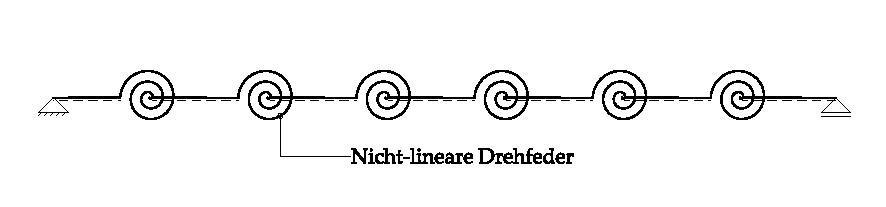
\includegraphics{index_files/mediabag/../imgs/Modell_Drehfeder.pdf}

}

\caption{\label{fig-modell_drehfeder}Modellierung als biegesteife Stäbe
gekoppelt mit Drehfedern}

\end{figure}%

Mit der Wahl der entsprechenden Federcharakteristiken stellen sich so
die passenden Resultate ein. Die Anwendung des Modells an
experimentellen Versuchen wird in den folgenden Kapiteln aufgegriffen.
Es lässt sich vorweggreifen, dass die Wahl der Federcharakteristik die
Krux des Systems darstellt.

Alternativ zur Modellierung mittels Drehfedern lässt sich das Verhalten
der Drehfeder mit einem Wegfederpaar abbilden. Dies erlaubt eine
Modellierung mittels den nicht-linearen Fachwerksstäben der Software
Statik-9 der Cubus AG. Dieser Ansatz wird lediglich im
Einführungsbeispiel berücksichtigt.

\begin{figure}[H]

\centering{

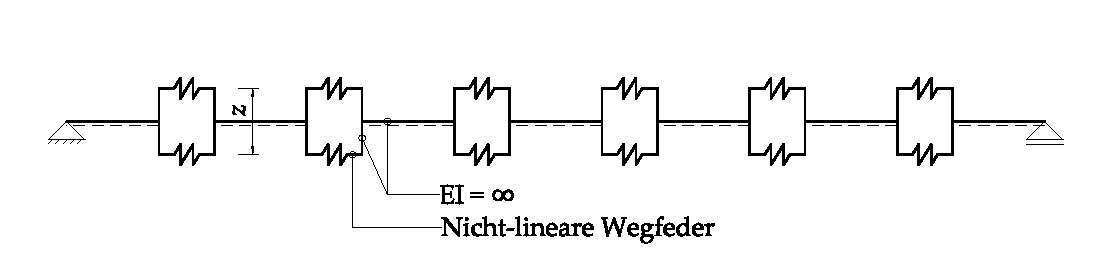
\includegraphics{index_files/mediabag/../imgs/Modell_Wegfeder.pdf}

}

\caption{\label{fig-modell_wegfeder}Modellierung als biegesteife Stäbe
gekoppelt mit einem Wegfederpaar}

\end{figure}%

\bookmarksetup{startatroot}

\chapter{Einführungsbeispiel}\label{einfuxfchrungsbeispiel}

Das Einführungsbeispiel verfolgt das Ziel das Modellverhalten zu
plausibilisieren. Die Eingabe der nicht-linearen Parameter in der
Statiksoftware liegt im Vordergrund.

Es werden die Verformungen des fiktiven Beispiels von Hand mittels der
Arbeitsgleichung, sowie numerisch mit der Stabstatik-Software ermittelt.
Das statische System ist in Abbildung~\ref{fig-kragarm-feder}
aufgezeigt. Das Beispiel ist mit einer Drehfeder versehen, welche eine
nicht-lineare Federcharakteristik aufweist. Es werden zwei Laststufen
betrachtet. Diese sind entsprechend gewählt, dass das nicht-lineare
Verhalten der Drehfeder zu tragen kommt.

\begin{figure}[H]

\centering{

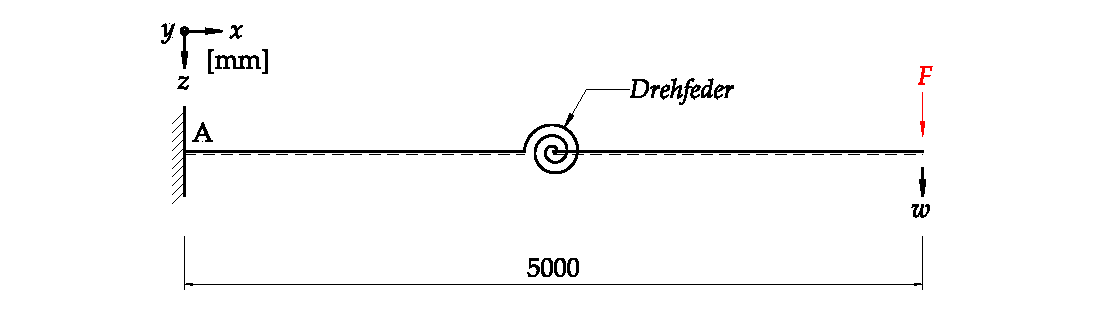
\includegraphics{index_files/mediabag/../imgs/Kragarm_system_Feder.pdf}

}

\caption{\label{fig-kragarm-feder}Statisches System des Kragarms}

\end{figure}%

Die folgenden Parameter fliessen in die Berechnungen ein. Beschrieben
sind die Abmessungen und Materialeigenschaften, sowie die beiden
Laststufen \(F_1\) und \(F_2\), wie auch die Federsteifigkeiten
\(k_{\varphi1}\) und \(k_{\varphi2}\).

$$
\begin{aligned}
E &= 10000.0\ \frac{\mathrm{N}}{\mathrm{mm}^{2}} \; 
 &F_{1} &= -10000.0\ \mathrm{N} \; 
 &F_{2} &= -21500.0\ \mathrm{N} \; 
\\[12pt]
 h &= 400.0\ \mathrm{mm} \; 
 &k_{\varphi_{1}} &= 100000.0\ \frac{\mathrm{N} \cdot \mathrm{m}}{\mathrm{rad}} \; 
 &k_{\varphi_{2}} &= 10000.0\ \frac{\mathrm{N} \cdot \mathrm{m}}{\mathrm{rad}} \; 
\\[12pt]
 l_{Kragarm} &= 5.0\ \mathrm{m} \; 
 &z &= 400.0\ \mathrm{mm} \; 
 &b &= 200.0\ \mathrm{mm} \; 
\\[12pt]
\end{aligned}
$$

Der Rechteckquerschnitt ist in Abbildung~\ref{fig-qs-kragarm}
aufgezeigt, dieser gilt für den gesamten Kragarm.

\begin{figure}[H]

\centering{

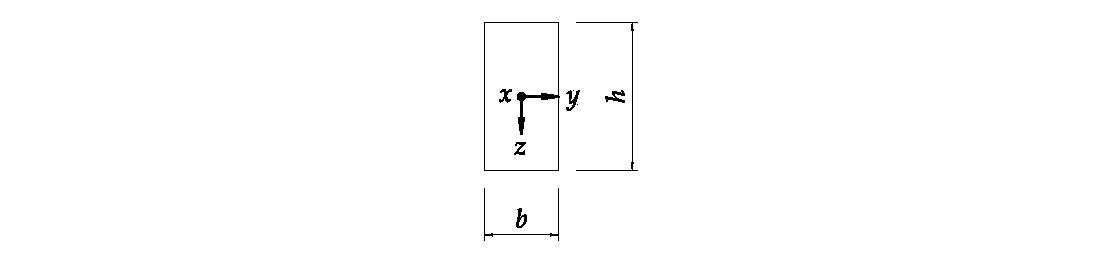
\includegraphics{index_files/mediabag/../imgs/Kragarm_querschnitt.pdf}

}

\caption{\label{fig-qs-kragarm}Fiktiver Querschnitt des Kragarms mit
durchwegs linear-elastischem Materialverhalten}

\end{figure}%

Die Entsprechende Federcharakteristik ist in
Abbildung~\ref{fig-springcharacteristic} zu sehen. Das Bilineare
Verhalten gilt für positive und negative Biegemomente um die
\(Y\)-Achse.

\begin{figure}[H]

{\centering \includegraphics{04_Kragarm_files/figure-pdf/cell-5-1-image.png}

}

\caption{image.png}

\end{figure}%

\begin{figure}[H]

\centering{

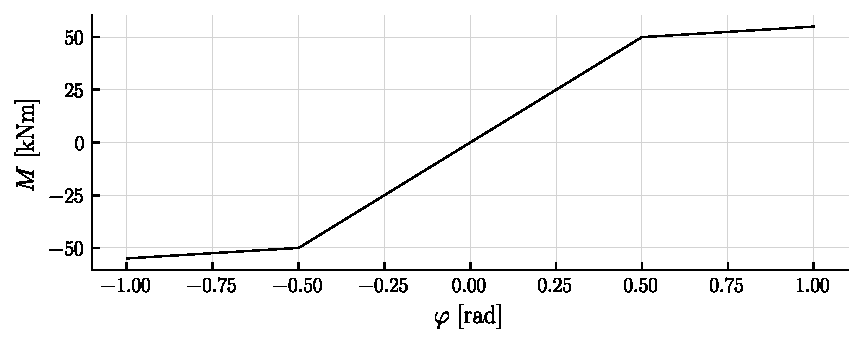
\includegraphics{index_files/mediabag/04_Kragarm_files/figure-pdf/fig-springcharacteristic-output-1.pdf}

}

\caption{\label{fig-springcharacteristic}Charakteristik der Drehfeder}

\end{figure}%

\section{Biegeverformung}\label{biegeverformung}

Zunächst werden die Biegeverformungen mittels der Differentialgleichung
für reine Biegeträger ermittelt. Dabei wird die Drehfeder
vernachlässigt. Das statische System, gezeigt in
Abbildung~\ref{fig-kragarm-sys} führt zu den Zustandslinien der
Schnittgrössen in der Abbildung~\ref{fig-skkragarmreal}.

\begin{figure}[H]

\centering{

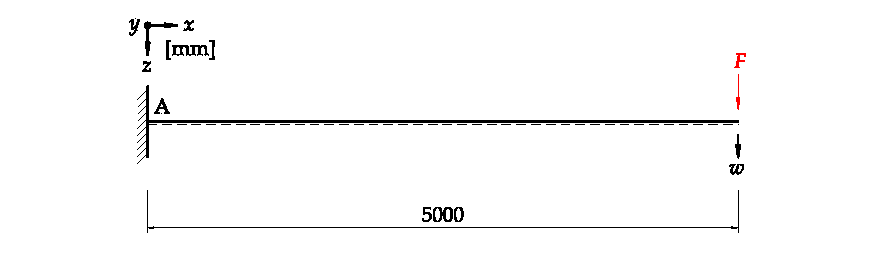
\includegraphics{index_files/mediabag/../imgs/Kragarm_System.pdf}

}

\caption{\label{fig-kragarm-sys}Statisches System des Kragarms}

\end{figure}%

\begin{figure}[H]

\centering{

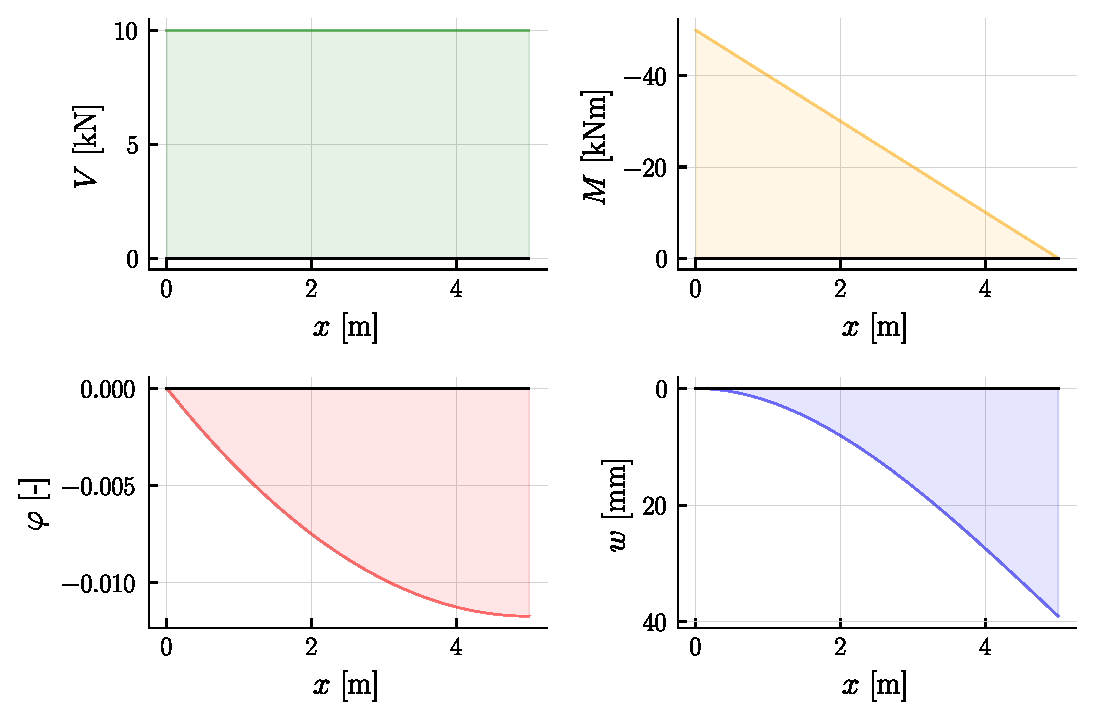
\includegraphics{index_files/mediabag/04_Kragarm_files/figure-pdf/fig-skkragarmreal-output-1.pdf}

}

\caption{\label{fig-skkragarmreal}Schnittkräfte des Systems aus
Abbildung~\ref{fig-kragarm-sys} für die Last \(F_1\)}

\end{figure}%

Die maximale Verformung am Endpunkt des Kragarms beträgt:

$$
\begin{aligned}
w_{bendingF1} &= 39.1\ \mathrm{mm} \;
\end{aligned}
$$

Das analoge Vorgehen führt für die Laststufe \(F_2\) zu den
Zustandslinien der Schnittgrössen gemäss der
Abbildung~\ref{fig-skkragarmreal_high}.

\begin{figure}[H]

\centering{

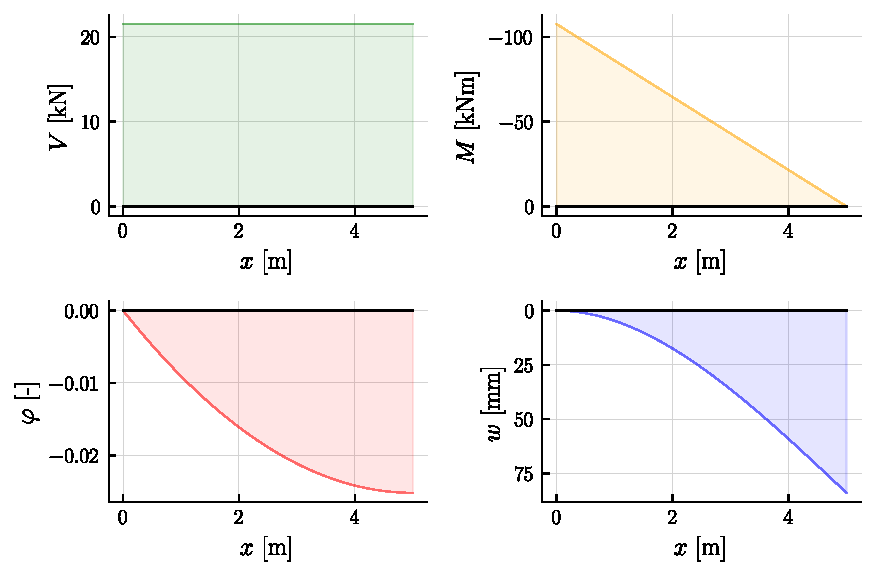
\includegraphics{index_files/mediabag/04_Kragarm_files/figure-pdf/fig-skkragarmreal_high-output-1.pdf}

}

\caption{\label{fig-skkragarmreal_high}Schnittkräfte des Systems aus
Abbildung~\ref{fig-kragarm-sys} für die Last \(F2\)}

\end{figure}%

Da ein durchwegs linear-elastisches Biegeverhalten vorausgesetzt wird,
entspricht der Faktor der Erhöhung des Verformung dem Quotient der
beiden Laststufen.

\[
\frac{w_{1,Bending,F2}}{w_{1,Bending,F1}} = \frac{F_2}{F_1}
\]

Dabei entspricht die maximale Biegeverformung am Ende des Kragarms:

$$
\begin{aligned}
w_{bendingF2} &= 84.0\ \mathrm{mm} \;
\end{aligned}
$$

\section{Verformung der Drehfeder}\label{verformung-der-drehfeder}

Zur Bestimmung der Verformung am Ende des Kragarms des Systems mit der
Drehfeder wird die Arbeitsgleichung angewendet. Dazu wird an einem
virtuellen System eine Einzellast eingeführt, an der Stelle an dem die
Verformung bestimmt werden soll. Dargestellt ist dies in
Abbildung~\ref{fig-kragarm-sys-virtuell}.

\begin{figure}[H]

\centering{

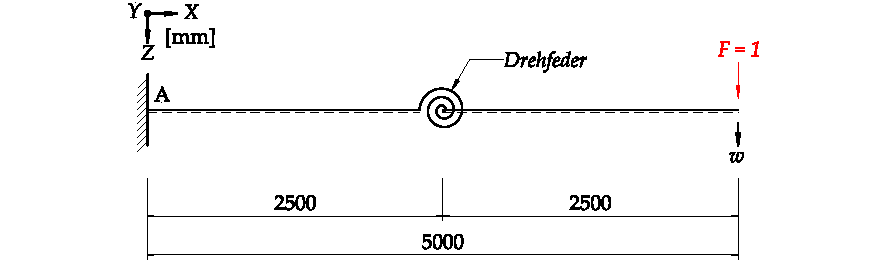
\includegraphics{index_files/mediabag/../imgs/Kragarm_system_feder_virtuell.pdf}

}

\caption{\label{fig-kragarm-sys-virtuell}Statisches System des Kragarms
im virtuellen Kräftezustand}

\end{figure}%

Die entsprechenden Verläufe der Querkraft und des Biegemoments zeigt die
Abbildung~\ref{fig-sk-kragarm-virtuell} für das virtuelle System.

\begin{figure}[H]

\centering{

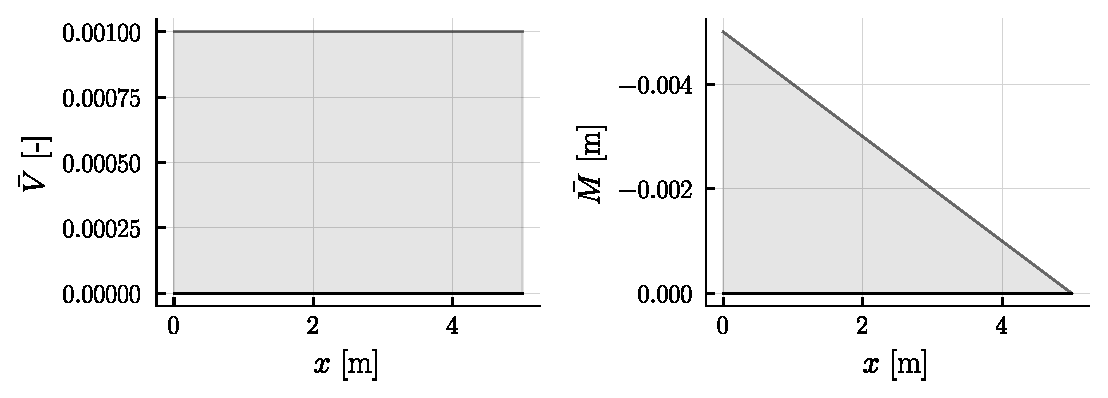
\includegraphics{index_files/mediabag/04_Kragarm_files/figure-pdf/fig-sk-kragarm-virtuell-output-1.pdf}

}

\caption{\label{fig-sk-kragarm-virtuell}Schnittkräfte des virtuellen
Systems aus Abbildung~\ref{fig-kragarm-sys-virtuell}}

\end{figure}%

Die Verformung der Drehfeder kann abschliessend mit der folgenden
Gleichung bestimmt werden.

\[
w_{Spring} = \bar{M} \frac{M}{k_\varphi} = \bar{M} \varphi
\]

Die Verdrehung lässt sich aus der Federcharakteristik mit dem
Biegemoment an der Stelle der Drehfeder bestimmen. Die
Abbildung~\ref{fig-feder-force} zeigt die Position der Laststufen im
Diagramm.

\begin{figure}[H]

\centering{

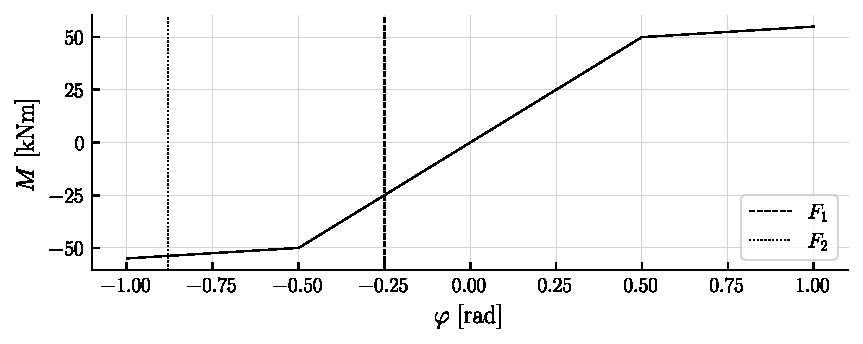
\includegraphics{index_files/mediabag/04_Kragarm_files/figure-pdf/fig-feder-force-output-1.pdf}

}

\caption{\label{fig-feder-force}Charakteristik der Drehfeder mit
Bestimmung der Verdrehung anhand der Laststufen}

\end{figure}%

Angewendet auf das System der Abbildung~\ref{fig-kragarm-feder} folgen
für die beiden Laststufen die Deformationen der Drehfeder zu:

$$
\begin{aligned}
w_{spring_{F1}} &= 625.0\ \mathrm{mm} \; 
 &w_{spring_{F2}} &= 2201.3\ \mathrm{mm} \;
\end{aligned}
$$

Dazu gilt es den Anteil aus der Biegeverformung zu addieren. Die totale
Verformung folgt zu:

$$
\begin{aligned}
w_{tot_{F1}} &= w_{spring_{F1}} + w_{bendingF1}  = 625.0\ \mathrm{mm} + 39.1\ \mathrm{mm} &= 664.1\ \mathrm{mm}  
\\[12pt]
w_{tot_{F2}} &= w_{spring_{F2}} + w_{bendingF2}  = 2201.3\ \mathrm{mm} + 84.0\ \mathrm{mm} &= 2285.2\ \mathrm{mm}  
\end{aligned}
$$

\section{Stabstatikmodell}\label{stabstatikmodell}

Das statische System, gemäss Abbildung~\ref{fig-kragarm-feder}, wird
mittels der Statiksoftware AxisVM X7 modelliert. Dazu wird die Drehfeder
als Federelement modelliert und in der \(YY\)-Dimension mit der
Federcharakteristik ergänzt. Die angeschlossenen Stäbe sind mit
entsprechendem Querschnitt und der entsprechenden Biegesteifigkeit
modelliert.

Die Deformationen in \(Z\)-Richtung sind in
Abbildung~\ref{fig-kragarm-drehfeder-10} und
Abbildung~\ref{fig-kragarm-drehfeder-215}

\begin{figure}[H]

\centering{

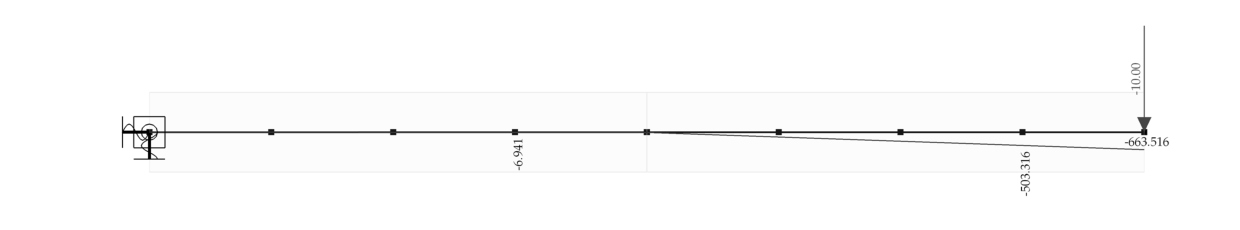
\includegraphics{index_files/mediabag/../imgs/Kragarm_drehfeder_10.pdf}

}

\caption{\label{fig-kragarm-drehfeder-10}Verformungen in \(z\) für
\(F_1\) aus AxisVM mit Drehfedermodell}

\end{figure}%

Das Modell liefert für die erste Laststufe die Gesamtverformung von:

\[
w_{1,tot,F1} = 663.5 \text{mm}
\]

\begin{figure}[H]

\centering{

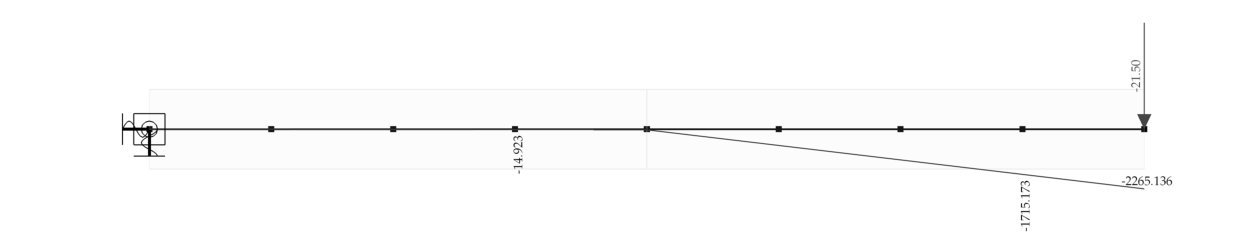
\includegraphics{index_files/mediabag/../imgs/Kragarm_drehfeder_215.pdf}

}

\caption{\label{fig-kragarm-drehfeder-215}Verformungen in \(z\) für
\(F_2\) aus AxisVM mit Drehfedermodell}

\end{figure}%

So wie für die zweite Laststufe folgt die Gesamtverformung zu:

\[
w_{1,tot,F2} = 2265.1 \text{mm}
\]

Das Modell liefert die annähernd gleichen Resultate wie die
Handrechnung. Die Genauigkeit ist zufriedenstellend.

\subsection{Modellierungsalternative
Wegfeder}\label{modellierungsalternative-wegfeder}

Wie bereits in Kapitel~\ref{sec-modellvorstellung} aufgezeigt, lässt
sich das Verhalten der Drehfeder mit einem Wegfederpaar abbilden. Dazu
wird in einem ersten Schritt die Drehfedercharakteristik in eine
Wegfedercharakteristik umgerechnet. Als Grundlage dient die Modellierung
gemäss Abbildung~\ref{fig-verdrehung_verformung}. Die Abbildung zeigt
die kinematische Relation eines reinen Biegeelements.

\begin{figure}[H]

\centering{

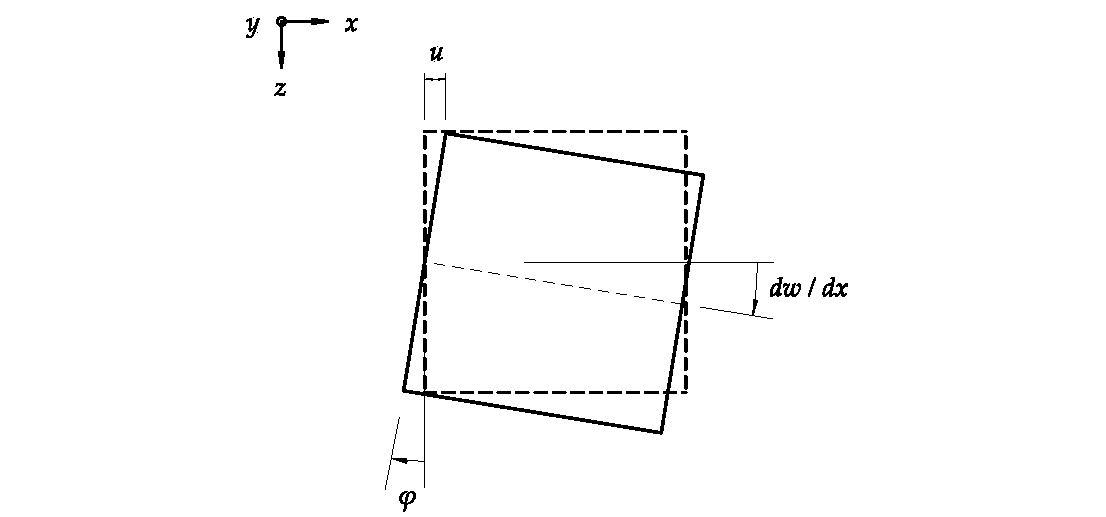
\includegraphics{index_files/mediabag/../imgs/Skizze_Verdrehung_Verformung.pdf}

}

\caption{\label{fig-verdrehung_verformung}Kinematische Relation eines
reinen Biegeelements}

\end{figure}%

Mittels den folgenden Gleichungen lässt sich so die
Wegfedercharakteristik bestimmen. Der Abstand zwischen dem Wegfederpaar
wird mit \(z\) beschrieben.

\[
F = \frac{M}{z}
\]

\[
u = \frac{\tan(\varphi) \cdot z}{2} \simeq \frac{\varphi \cdot z}{2}
\]

Durch die Berücksichtigung der trigonometrischen Funktion ist der
Verlauf nicht exakt bilinear. Eine Approximation mit einem bilinearen
Verlauf führt zu beträchtlichen Abweichungen im Bereich der zweiten
Laststufe \(F_2\). Dies ist auf die geringe Neigung, bzw.
\(k_{\varphi_2}\) der Drehfedercharakteristik im oberen Lastniveau
zurückzuführen.

Die umgerechnete Wegfedercharakteristik ist in
Abbildung~\ref{fig-wegfeder-force} aufgezeigt.

\begin{figure}[H]

\centering{

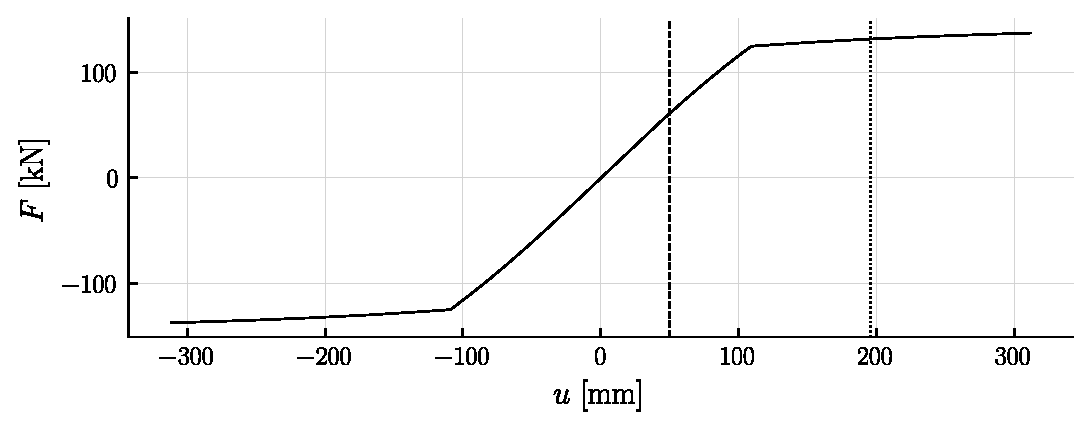
\includegraphics{index_files/mediabag/04_Kragarm_files/figure-pdf/fig-wegfeder-force-output-1.pdf}

}

\caption{\label{fig-wegfeder-force}Charakteristik der Wegfeder}

\end{figure}%

Die Resultate mit dem Modell sind in der Abbildung~\ref{fig-f1-wegfeder}
und Abbildung~\ref{fig-f2-wegfeder} gezeigt.

\begin{figure}[H]

\centering{

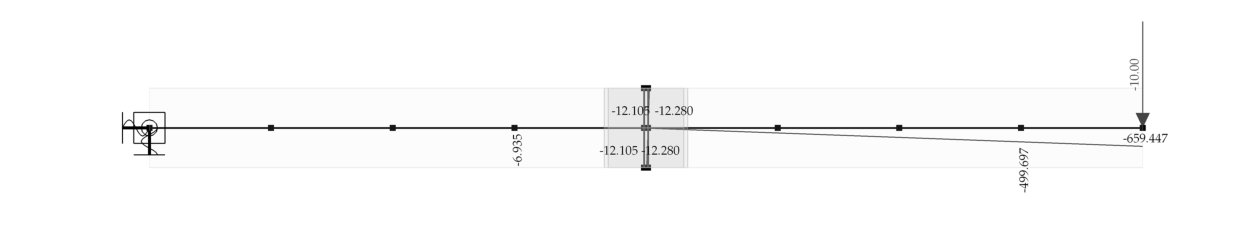
\includegraphics{index_files/mediabag/../imgs/Kragarm_wegfeder_10.pdf}

}

\caption{\label{fig-f1-wegfeder}Verformungen in \(z\) für \(F_1\) aus
AxisVM mit Wegfedermodell}

\end{figure}%

Die maximale Verformung in \(Z\)-Richtung ist für die Laststufe \(1\):

\[
w_{1,tot,F1} = 655 \text{mm}
\]

Und für die Laststufe \(2\):

\[
w_{1,tot,F2} = 2137.8 \text{mm}
\]

Hier zeigt sich eine Abweichung. Diese lässt sich auf die numerisch
approximierte Modellierung der Wegfederbeziehung zurückführen.

\begin{figure}[H]

\centering{

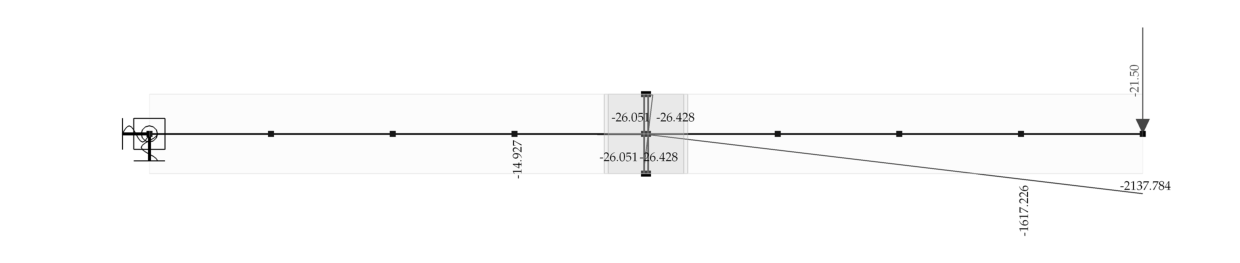
\includegraphics{index_files/mediabag/../imgs/Kragarm_wegfeder_215.pdf}

}

\caption{\label{fig-f2-wegfeder}Verformungen in \(z\) für \(F_2\) aus
AxisVM mit Wegfedermodell}

\end{figure}%

\section{Zusammenfassung}\label{zusammenfassung}

Das Einführungsbeispiel zeigt die Präzision der Modellierung mittels dem
Drehfedermodell. Sowie ermöglicht die simple Aufgabenstellung das
Nachvollziehen der Resultate.

\bookmarksetup{startatroot}

\chapter{Modellverifizierung}\label{modellverifizierung}

In diesem Kapitel werden die beiden Versuche aus der Vorarbeit
{[}\citeproc{ref-gitz_ansatze_2024}{1}{]} mit einem Drehfedermodell,
gemäss dem Beschrieb in Kapitel~\ref{sec-modellvorstellung},
nachgerechnet. Dazu wird eine feine Stabunterteilung gewählt, um das
Verformungsverhalten präzise abzubilden. Detaillierte Berechnungen und
Versuchsbeschriebe, welche als Grundlagen für die Modellierung dienen,
sind in {[}\citeproc{ref-gitz_ansatze_2024}{1}{]} zu finden.
Grundsätzlich gilt, dass für den Betonstahl bilineare
Spannungs-Dehnungs-Beziehungen hinterlegt sind und für den Beton ein
elastisch-ideal-plastisches Gesetz mit Berücksichtigung der
Zugfestigkeit.

\section{Dreipunktbiegeversuch}\label{dreipunktbiegeversuch}

Der Dreipunktbiegeversuch ist der dritte Versuch der Serie A in der
zweiten Versuchsanordnung aus
{[}\citeproc{ref-jager_versuche_2006}{2}{]}, kurz betitelt mit A3V2.
Dieser ist mit einer durchegehenden Längsbewehrung im Zugbereich
bewehrt. Die Schubdübel sind nicht durchgängig verlegt. Dargestellt ist
das Bewehrungslayout in der Abbildung~\ref{fig-bewehrung_a3v2}.

\begin{figure}[H]

\centering{

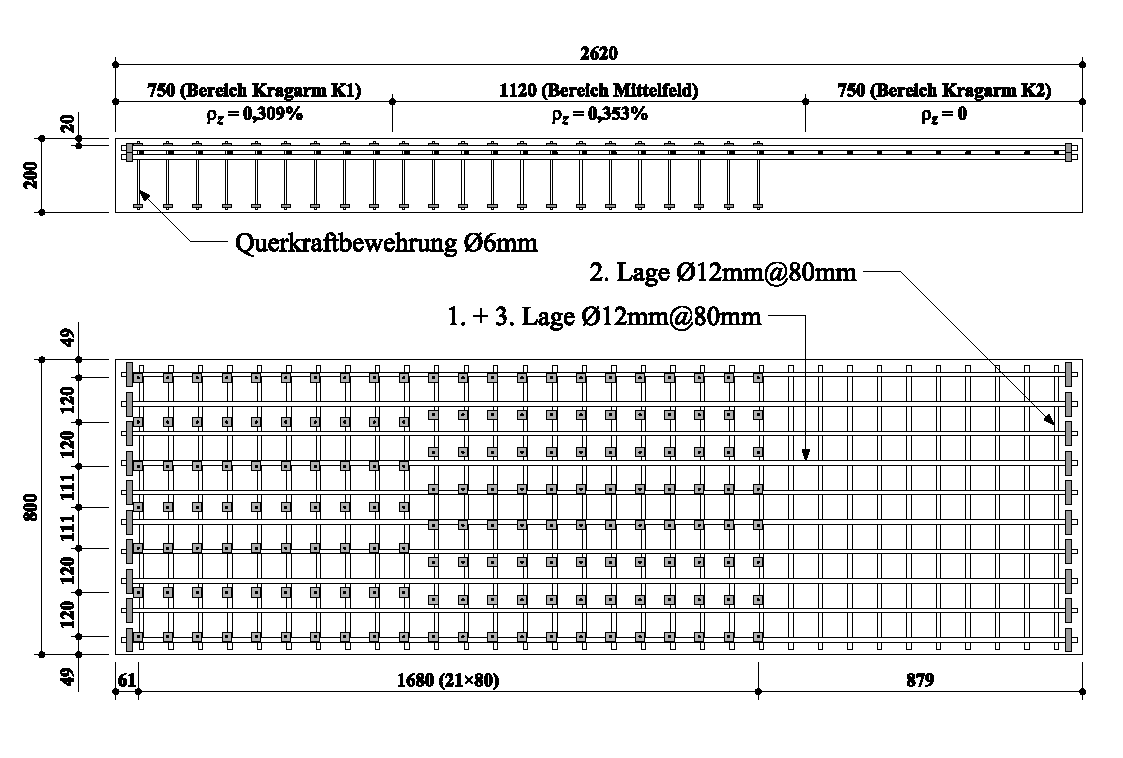
\includegraphics{index_files/mediabag/../imgs/bewehrung_a3v2.pdf}

}

\caption{\label{fig-bewehrung_a3v2}Bewehrunslayout des Versuchs A3V2,
Zeichnung entnommen aus {[}\citeproc{ref-jager_versuche_2006}{2}{]}}

\end{figure}%

Das statische System des Versuchs ist in Abbildung~\ref{fig-system_a3v2}
dargestellt. Das Eigengewicht wird vernachlässigt, da die
Verformungsmessungen nach dem Einbau des Versuchs beginnen, bzw. erst
bei Belastungsbeginn mit der Einzellast.

\begin{figure}[H]

\centering{

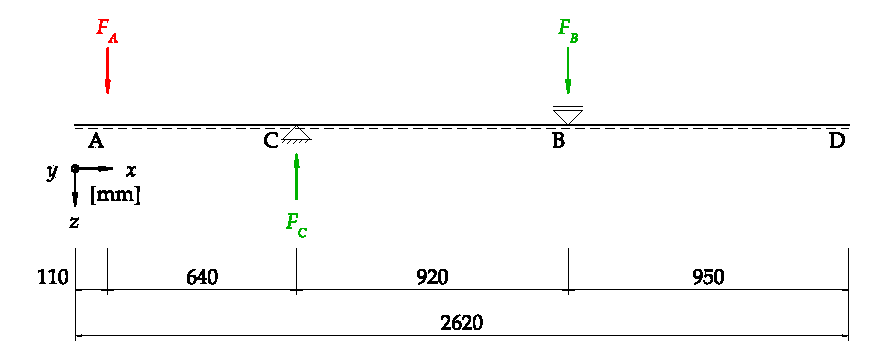
\includegraphics{index_files/mediabag/../imgs/A3V2_system.pdf}

}

\caption{\label{fig-system_a3v2}Statisches System des Versuchs A3V2}

\end{figure}%

Die Abbildung~\ref{fig-qs_a3v2} zeigt den Querschnitt des Versuchs mit
der entsprechenden Bewehrungsführung.

\begin{figure}[H]

\centering{

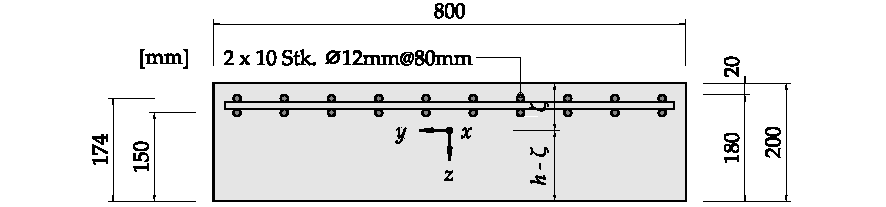
\includegraphics{index_files/mediabag/../imgs/QS_Versuch_A3.pdf}

}

\caption{\label{fig-qs_a3v2}Querschnitt des Versuchs A3V2, Zeichnung
entnommen aus {[}\citeproc{ref-gitz_ansatze_2024}{1}{]}}

\end{figure}%

\subsection{Drehfedercharakteristik}\label{drehfedercharakteristik}

Als erster Eingabeparamter in das Drehfedermodell dient die
Momenten-Krümmungs-Beziehung. Für den Querschnitt ist die nicht-lineare
Beziehung in der Abbildung~\ref{fig-mchi_a3v2} gezeigt. Detaillierte
Berechnungen sind in der Vorarbeit
{[}\citeproc{ref-gitz_ansatze_2024}{1}{]} zu finden.

\begin{figure}[H]

\centering{

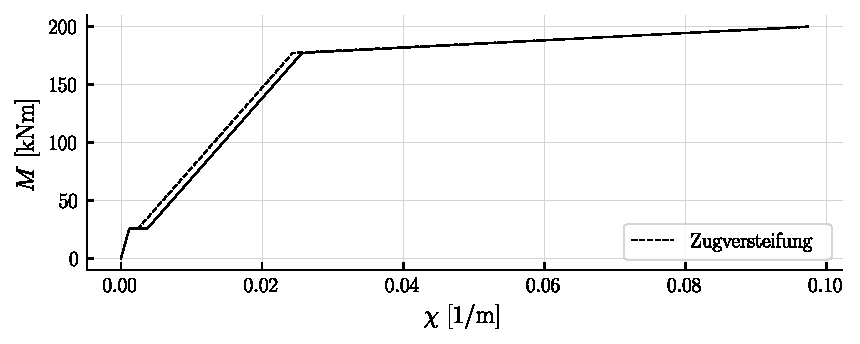
\includegraphics{index_files/mediabag/05_Versuchsnachrechnung_VM1_files/figure-pdf/fig-mchi_a3v2-output-1.pdf}

}

\caption{\label{fig-mchi_a3v2}Momenten-Krümmungs-Beziehung des
Dreipunktbiegeversuchs, übernommen aus
{[}\citeproc{ref-gitz_ansatze_2024}{1}{]}}

\end{figure}%

$$
\begin{aligned}
l_{E} &= 10.0\ \mathrm{mm} \; \;\textrm{(Elementlänge des Biegesteifen Stabs)}
\end{aligned}
$$

\subsection{Wegfedercharakteristik}\label{wegfedercharakteristik}

\subsubsection{Schiebung}\label{schiebung}

Als Grundlage zur Modellierung der Schubverformungen dient das
Spannungsfeld-Modell in Abbildung~\ref{fig-spannungsfelder_a3v2}. Dabei
wird vorausgesetzt, dass sämtliche Dehnung des Systems in vertikaler
Richtung lediglich aus der Stabdehnung der Schubbewehrung erfolgt. Das
Ziel ist es ein Kraft-Verformungs-Diagramm, bzw. eine
Wegfedercharakteristik zu ermitteln.

\begin{figure}[H]

\centering{

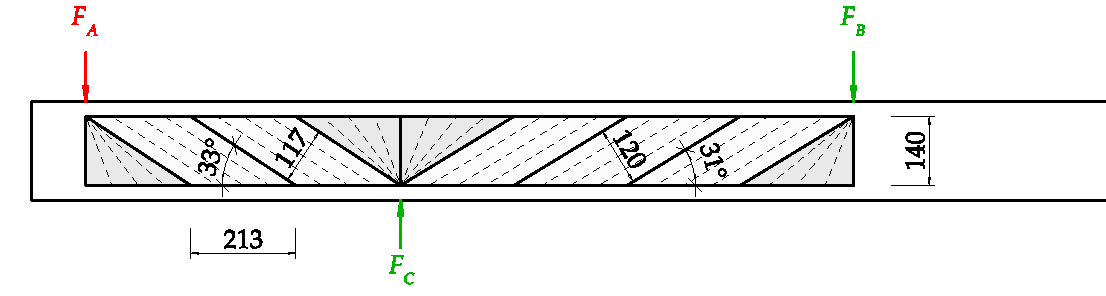
\includegraphics{index_files/mediabag/../imgs/Spannungsfelder_flach.pdf}

}

\caption{\label{fig-spannungsfelder_a3v2}Einteilung in Spannungsfelder
des Versuchs A3V2, Zeichnung entnommen aus
{[}\citeproc{ref-gitz_ansatze_2024}{1}{]}}

\end{figure}%

Durch die Einteilung in Spannungsfelder kann die Anzahl an mitwirkenden
Schubdübeln bestimmt werden. Mit der Querschnittsfläche der mitwirkenden
Dübel kann das nicht-lineare Spannungs-Dehnungs-Verhalten in ein
Kraft-Verformungs-Diagramm bzw. in eine Wegfedercharakteristik
umgewandelt werden. Die bekannte Dehnung aus der Stahlkennlinie wird
über den Hebelarm der inneren Kräfte zu einer Verformung umgewandelt.
Wichtig dabei ist die Elementlänge der biegesteifen Stäbe im FEM-Modell.
Dazu wird die Verformung um den Faktor gemäss der folgenden Gleichung
reduziert, bzw. die Steifigkeit der Feder um diesen Faktor erhöht.

\[
\gamma_{E} = \frac{z \cdot \cot(\theta)}{n_{E}}
\]

\(n_{E}\) steht für die Anzahl steifer Stabelemente

\begin{figure}[H]

\centering{

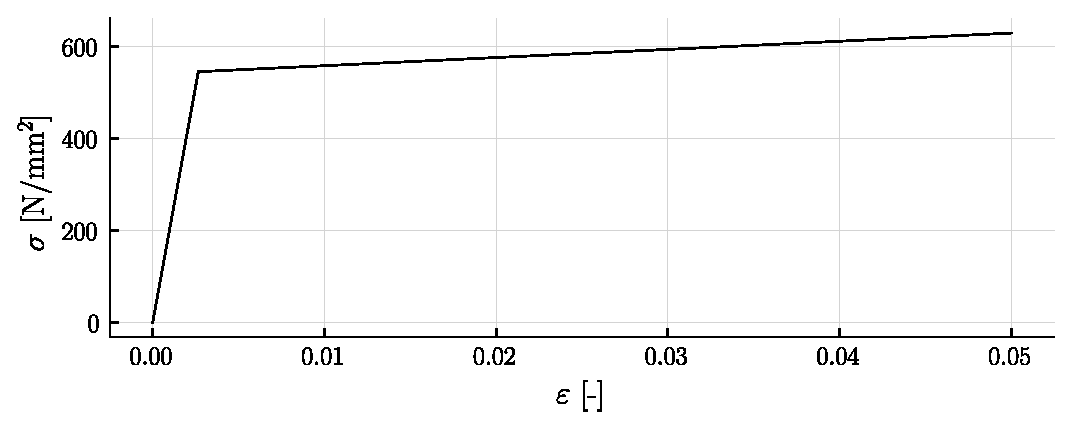
\includegraphics{index_files/mediabag/05_Versuchsnachrechnung_VM1_files/figure-pdf/fig-sigma-eps-a3v2-output-1.pdf}

}

\caption{\label{fig-sigma-eps-a3v2}Spannungs-Dehnungs-Beziehung der
Schubbewehrung, übernommen aus
{[}\citeproc{ref-gitz_ansatze_2024}{1}{]}}

\end{figure}%

Folgend sind die Parameter zur Bestimmung der Wegfedercharakteristik in
vertikaler Richtung gezeigt. Der gewählte Neigungswinkel der
Spannungsfelder \(\theta_{c3}\) gilt grundsätzlich nur im Bruchzustand.
Als Approximation wird die daraus bestimmte Wegfedercharakteristik für
sämtliche Laststufen angesetzt. Dies führt zu Abweichungen im Lastniveau
unterhalb der Traglast, sofern die Schubverformung einen signifikanten
Einfluss an der der Gesamtverformung liefern.

$$
\begin{aligned}
\oslash_{sw_{A3V2}} &= 6.0\ \mathrm{mm} \; 
 &S_{sw_{A3V2}} &= 80.0\ \mathrm{mm} \; 
 &b_{w_{A3V2}} &= 800.0\ \mathrm{mm} \; 
\\[12pt]
 E_{sw_{A3V2}} &= 205000.0\ \frac{\mathrm{N}}{\mathrm{mm}^{2}} \; 
 &E_{sh_{A3V2}} &= 1774.5\ \frac{\mathrm{N}}{\mathrm{mm}^{2}} \; 
 &z_{A3V2} &= 140.0\ \mathrm{mm} \; 
\\[12pt]
 \theta_{c3_{A3V2}} &= 34.3\ \mathrm{°} \; 
 &f_{su_{A3V2}} &= 630.0\ \frac{\mathrm{N}}{\mathrm{mm}^{2}} \;
\end{aligned}
$$

Die Querschnittsfläche der Schubbewehrung bestimmt sich zu:

$$
\begin{aligned}
A_{sw_{A3V2}} &= 7 \cdot \left( \frac{ \oslash_{sw_{A3V2}} }{ 2 } \right) ^{ 2 } \cdot \pi \; 
\end{aligned}
$$

$$
\begin{aligned}
A_{sw_{A3V2}} &= 197.9\ \mathrm{mm}^{2} \;
\end{aligned}
$$

Verschmiert über einen Meterstreifen:

$$
\begin{aligned}
a_{sw_{A3V2}} &= \frac{ A_{sw_{A3V2}} }{ S_{sw_{A3V2}} } \; 
\end{aligned}
$$

$$
\begin{aligned}
a_{sw_{A3V2}} &= 2474.0\ \frac{\mathrm{mm}^{2}}{\mathrm{m}} \;
\end{aligned}
$$

Der Querkraftwiderstand mit gewählter Neigung:

$$
\begin{aligned}
V_{Rd_{A3V2}} &= a_{sw_{A3V2}} \cdot z_{A3V2} \cdot \frac{ f_{su_{A3V2}} }{ \tan \left( \theta_{c3_{A3V2}} \right) } \; 
\end{aligned}
$$

$$
\begin{aligned}
V_{Rd_{A3V2}} &= 319.9\ \mathrm{kN} \;
\end{aligned}
$$

Der Reduktionsfaktor bestimmt sich zu:

$$
\begin{aligned}
\gamma_{E_{A3V2}} &= z_{A3V2} \cdot \frac{ 1 }{ \tan \left( \theta_{c3_{A3V2}} \right) } \cdot \frac{1} { l_{E} }  = 140\ \mathrm{mm} \cdot \frac{ 1 }{ \tan \left( 34\ \mathrm{°} \right) } \cdot \frac{1} { 10\ \mathrm{mm} } &= 21\  
\end{aligned}
$$

Die Abbildung~\ref{fig-wegfeder-schub-a3v2} zeigt das
Kraft-Verformungs-Verhalten für die Gelenke des Stabmodells in
vertikaler Richtung.

\begin{figure}[H]

\centering{

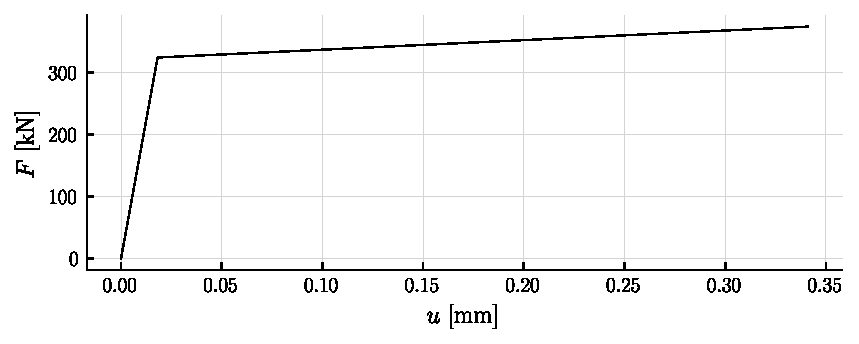
\includegraphics{index_files/mediabag/05_Versuchsnachrechnung_VM1_files/figure-pdf/fig-wegfeder-schub-a3v2-output-1.pdf}

}

\caption{\label{fig-wegfeder-schub-a3v2}Berechnete
Wegfedercharakteristik des Schubgelenks vom Versuch A3V2}

\end{figure}%

\subsection{Versuchsvergleich}\label{versuchsvergleich}

Mit den bestimmten Federcharakteristiken kann die Biegelinie des Systems
ermittelt werden unter Berücksichtigung der Schub- und Biegeverformungen
auf nicht-linearen Grundlagen. Die Abbildung~\ref{fig-fwa3v2} zeigt das
Last-Verformungs-Diagramm des Systems am Punkt \(w_1\). Das Modell
beschreibt den Verformungsverlauf zufriedenstellend.

\begin{figure}[H]

\centering{

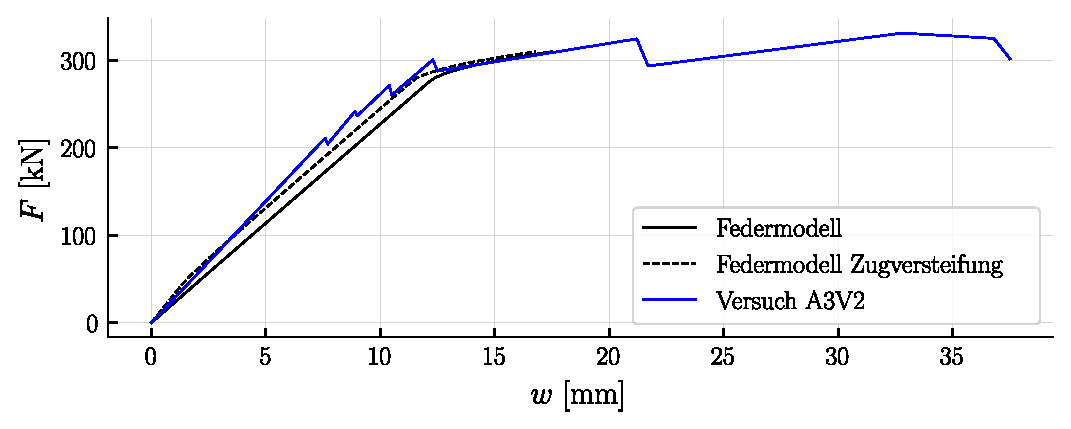
\includegraphics{index_files/mediabag/05_Versuchsnachrechnung_VM1_files/figure-pdf/fig-fwa3v2-output-1.pdf}

}

\caption{\label{fig-fwa3v2}Last-Verformungs-Verlauf am Punkt \(w_1\) mit
dem Federmodell und den Versuchsmessungen}

\end{figure}%

Der Verdrehungsverlauf in Abbildung~\ref{fig-phi-max-a3v2} lässt sich
ebenfalls direkt aus dem Modell exportieren. Durch die Ableitung des
Verlaufs resultiert der Krümmungsverlauf, dargestellt in
Abbildung~\ref{fig-chi-max-a3v2}.

\begin{figure}[H]

\centering{

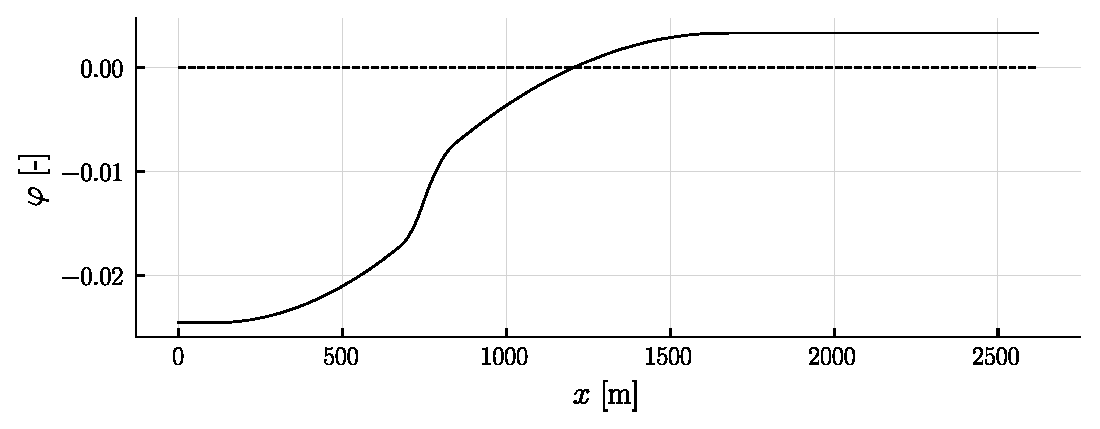
\includegraphics{index_files/mediabag/05_Versuchsnachrechnung_VM1_files/figure-pdf/fig-phi-max-a3v2-output-1.pdf}

}

\caption{\label{fig-phi-max-a3v2}Verdrehungsverlauf aus dem Federmodell
für die Höchstlast}

\end{figure}%

Der Krümmungsverlauf gibt Aufschluss über den Fliessbereich der
Bewehrung, bzw. über den Steifigkeitenverlauf entlang der Stabachse.

\begin{figure}[H]

\centering{

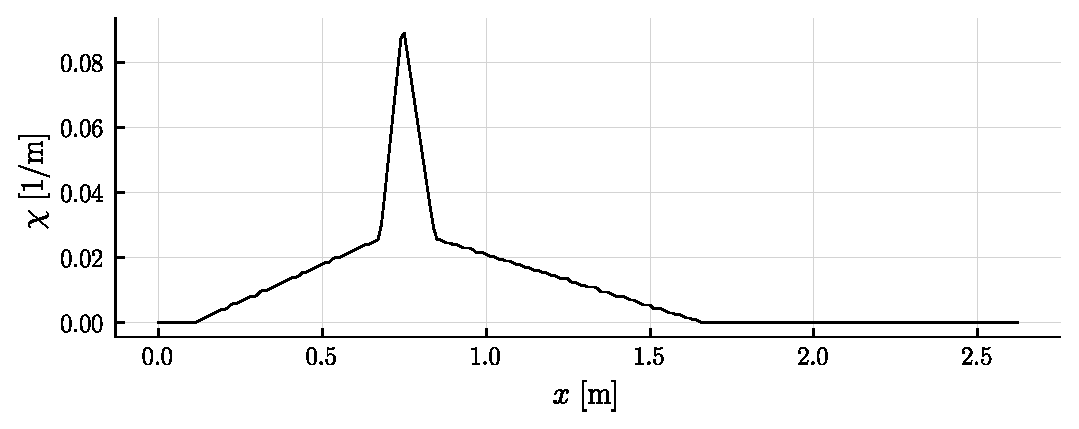
\includegraphics{index_files/mediabag/05_Versuchsnachrechnung_VM1_files/figure-pdf/fig-chi-max-a3v2-output-1.pdf}

}

\caption{\label{fig-chi-max-a3v2}Berechneter Krümmungsverlauf aus dem
Verdrehungsverlauf}

\end{figure}%

\newpage{}

\section{Vierpunktbiegeversuch}\label{vierpunktbiegeversuch}

Der Vierpunktbiegeversuch ist aus dem Paper
{[}\citeproc{ref-tue_einfluss_2019}{3}{]} entnommen. Auffallend bei
diesem Versuch ist die niedrig gehaltene Schubbewehrung. Dazu sind in
Längsrichtung Stäbe mit unterschiedlicher Güte verlegt.

\begin{figure}[H]

\centering{

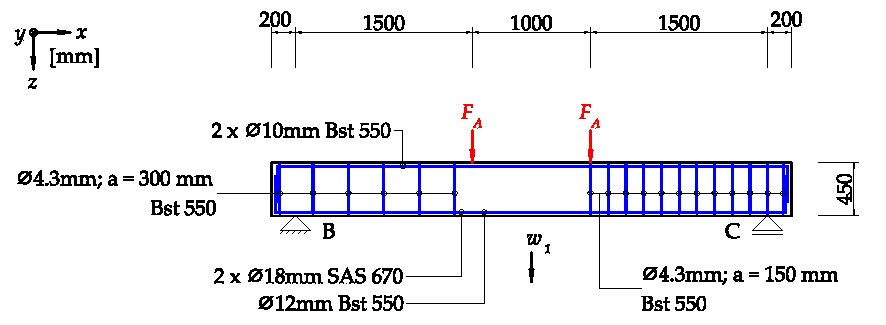
\includegraphics{index_files/mediabag/../imgs/versuchsskizze_14.pdf}

}

\caption{\label{fig-versuchsskizze-SV14}Bewehrungslayout des Versuchs
SV14, Zeichnung entnommen aus {[}\citeproc{ref-gitz_ansatze_2024}{1}{]}}

\end{figure}%

Der Querschnitt ist in der Abbildung~\ref{fig-QS-SV14} gezeigt. Die
Druckbewehrung wird vernachlässigt.

\begin{figure}[H]

\centering{

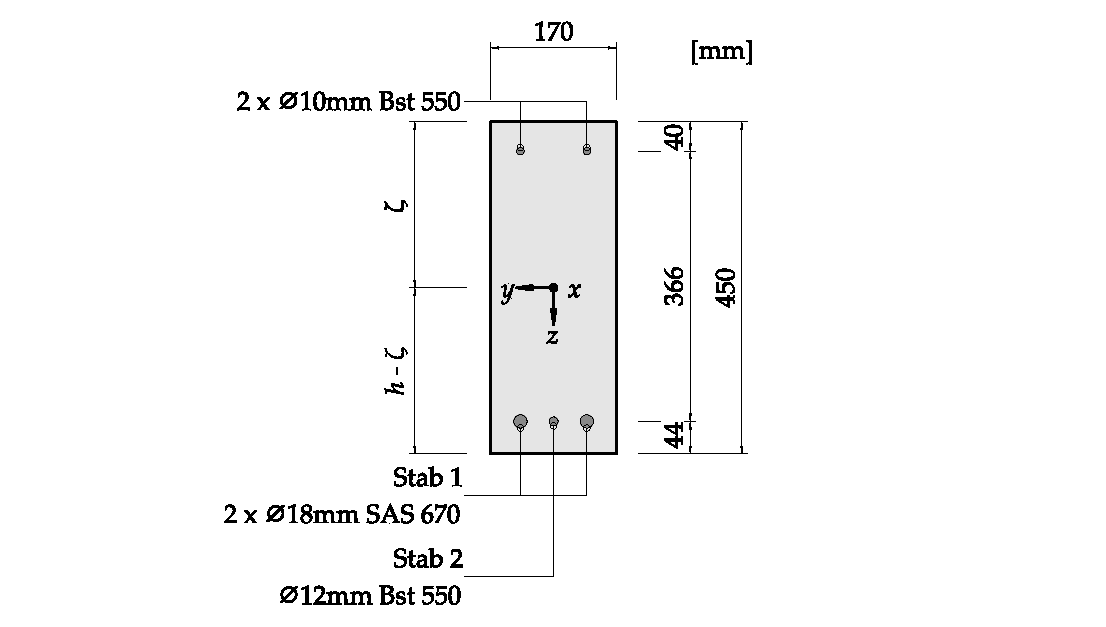
\includegraphics{index_files/mediabag/../imgs/QS_Versuch14.pdf}

}

\caption{\label{fig-QS-SV14}Querschnitt des Versuchs SV14, Zeichnung
entnommen aus {[}\citeproc{ref-gitz_ansatze_2024}{1}{]}}

\end{figure}%

Das statische System ist in der Abbildung~\ref{fig-system-SV14} gezeigt.
Auch hier wird das Eigengewicht, wie im Versuch A3V2, vernachlässigt.
Die gemessene und rechnerisch bestimmte Verformung gelten für den
Mittelspunkt, beschrieben mit \(w_1\).

\begin{figure}[H]

\centering{

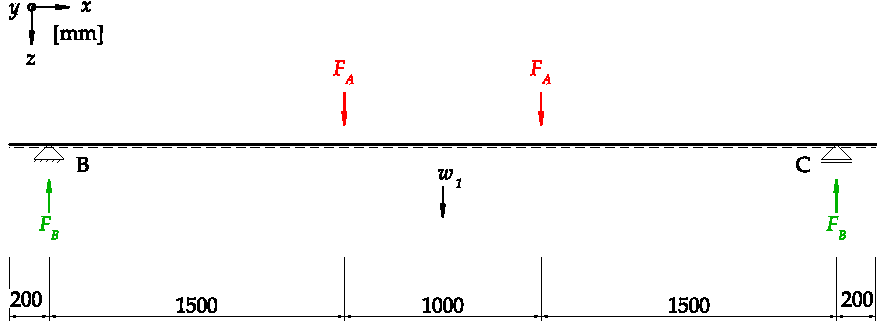
\includegraphics{index_files/mediabag/../imgs/statisches_system_14.pdf}

}

\caption{\label{fig-system-SV14}Statisches System des Versuchs SV14,
Zeichnung entnommen aus {[}\citeproc{ref-gitz_ansatze_2024}{1}{]}}

\end{figure}%

\subsection{Schnittgrössen}\label{schnittgruxf6ssen}

\subsection{Drehfedercharakteristik}\label{drehfedercharakteristik-1}

Als Grundlage für die Drehfedercharakteristik gilt die
Momenten-Krümmungs-Beziehung. Für den Querschnitt des Versuchs SV14 gilt
die Beziehung gemäss Abbildung~\ref{fig-mchi_sv14}. Für detaillierte
Berechnungen ist die Vorarbeit {[}\citeproc{ref-gitz_ansatze_2024}{1}{]}
zu konsultieren.

\begin{figure}[H]

\centering{

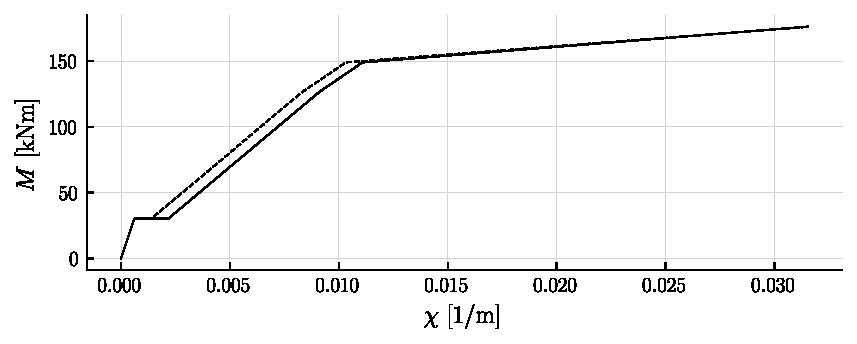
\includegraphics{index_files/mediabag/05_Versuchsnachrechnung_VM1_files/figure-pdf/fig-mchi_sv14-output-1.pdf}

}

\caption{\label{fig-mchi_sv14}Momenten-Krümmungs-Beziehung des
Vierpunktbiegeversuchs, übernommen aus
{[}\citeproc{ref-gitz_ansatze_2024}{1}{]}}

\end{figure}%

\subsection{Versatzmass}\label{versatzmass}

In diesem Kapitel wird das Versatzmass bestimmt. Bzw. im Vergleich mit
der Vertiefungsarbeit {[}\citeproc{ref-gitz_ansatze_2024}{1}{]}
berichtigt. Es wird vom Versuch lediglich die starke Seite betrachtet,
da durch Verstärkungsmassnahmen diese bis zum Versagen gebracht wird.

Die Materialeigenschaften sind in
{[}\citeproc{ref-marienhutte_produktdatenblatt_b550bpdf_nodate}{4}{]}
ersichtlich.

$$
\begin{aligned}
V_{exp_{sv14}} &= 105.0\ \mathrm{kN} \; 
 &z_{SV14} &= 359.0\ \mathrm{mm} \; 
 &\oslash_{sw_{SV14}} &= 4.3\ \mathrm{mm} \; 
\\[12pt]
 b_{w_{SV14}} &= 170.0\ \mathrm{mm} \; 
 &S_{sw_{SV14}} &= 150.0\ \mathrm{mm} \; 
 &f_{su_{SV14}} &= 715.0\ \frac{\mathrm{N}}{\mathrm{mm}^{2}} \; 
\\[12pt]
 \theta_{c3_{SV14}} &= 25.6\ \mathrm{°} \; 
 &F_{B} &= 105.0\ \mathrm{kN} \; 
 &F_{A} &= 105.0\ \mathrm{kN} \; 
\\[12pt]
\end{aligned}
$$

Mit den Parametern, bzw. der Neigung der Betondruckdiagonale resultiert
der nötige Querkraftwiderstand.

$$
\begin{aligned}
A_{sw_{SV14}} &= 2 \cdot \left( \frac{ \oslash_{sw_{SV14}} }{ 2 } \right) ^{ 2 } \cdot \pi \; 
\end{aligned}
$$

$$
\begin{aligned}
A_{sw_{SV14}} &= 29.0\ \mathrm{mm}^{2} \;
\end{aligned}
$$

$$
\begin{aligned}
a_{sw_{SV14}} &= \frac{ A_{sw_{SV14}} }{ S_{sw_{SV14}} } \; 
\end{aligned}
$$

$$
\begin{aligned}
a_{sw_{SV14}} &= 193.6\ \frac{\mathrm{mm}^{2}}{\mathrm{m}} \;
\end{aligned}
$$

$$
\begin{aligned}
V_{Rd_{SV14}} &= a_{sw_{SV14}} \cdot z_{SV14} \cdot \frac{ f_{su_{SV14}} }{ \tan \left( \theta_{c3_{SV14}} \right) } \; 
\end{aligned}
$$

$$
\begin{aligned}
V_{Rd_{SV14}} &= 103.8\ \mathrm{kN} \;
\end{aligned}
$$

Die Spannungsfeldeinteilung ist in der
Abbildung~\ref{fig-spannungsfelder_sv14} gezeigt. Die Feldneigung ist
näherungsweise an die berechnete Neigung angepasst.

\begin{figure}[H]

\centering{

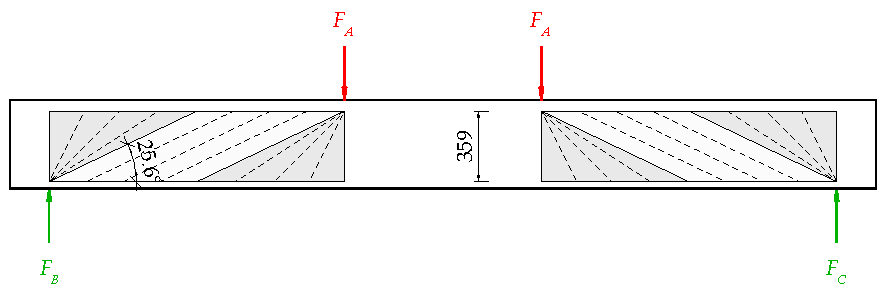
\includegraphics{index_files/mediabag/../imgs/SV14_spannungsfelder.pdf}

}

\caption{\label{fig-spannungsfelder_sv14}Einteilung in Spannungsfelder}

\end{figure}%

Wird nun Gleichgewicht an den entsprechenden Spannungsfeldern ausgeübt,
so lässt sich der Zug- und Druckkraftverlauf bestimmen.

\begin{figure}[H]

\centering{

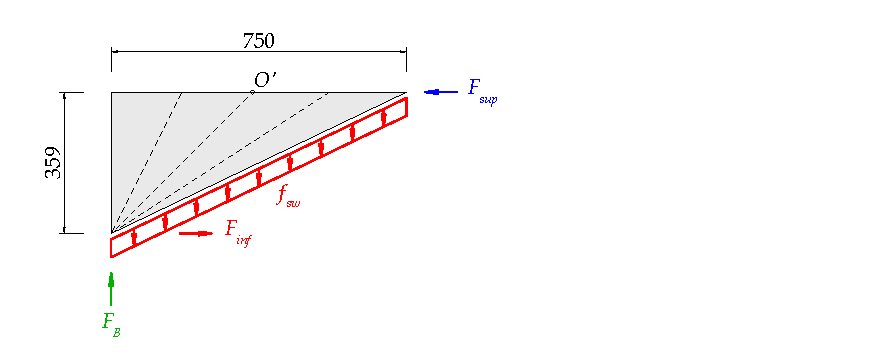
\includegraphics{index_files/mediabag/../imgs/SV14_skd_1.pdf}

}

\caption{\label{fig-skd_1_spannungsfelder_sv14}Schnittkörperdiagramm des
zentrierten Fächers}

\end{figure}%

Die Kraft im Untergurt:

$$
\begin{aligned}
F_{inf_{1}} &= F_{B} \cdot \frac{ z_{SV14} }{ \tan \left( \theta_{c3_{SV14}} \right) } \cdot \frac{1} { 2 } \cdot \frac{1} { z_{SV14} } \; 
\end{aligned}
$$

$$
\begin{aligned}
F_{inf_{1}} &= 109.7\ \mathrm{kN} \; 
\end{aligned}
$$

Die Kraft im Obergurt:

$$
\begin{aligned}
F_{sup_{1}} &= F_{inf_{1}} \; 
\end{aligned}
$$

$$
\begin{aligned}
F_{sup_{1}} &= 109.7\ \mathrm{kN} \; 
\end{aligned}
$$

Der Anteil an der Schubbewehrung:

$$
\begin{aligned}
f_{sw_{1}} &= \frac{ F_{B} }{ z_{SV14} } \cdot \frac{1} { \tan \left( \theta_{c3_{SV14}} \right) } \; 
\end{aligned}
$$

$$
\begin{aligned}
f_{sw_{1}} &= 611.0\ \frac{\mathrm{kN}}{\mathrm{m}} \;
\end{aligned}
$$

\begin{figure}[H]

\centering{

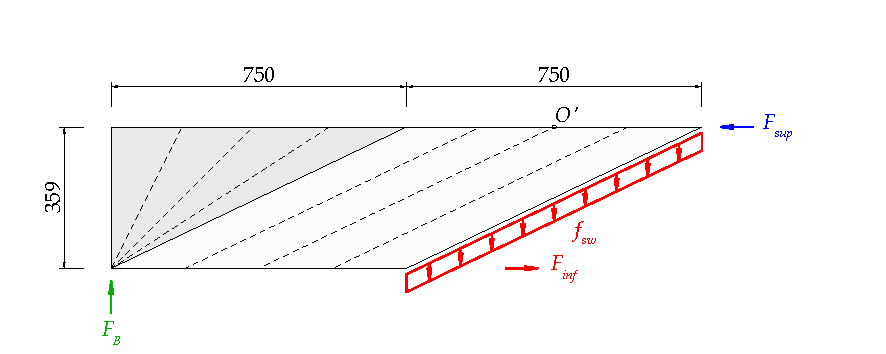
\includegraphics{index_files/mediabag/../imgs/SV14_skd_2.pdf}

}

\caption{\label{fig-skd_2_spannungsfelder_sv14}Schnittkörperdiagramm des
Parallelfelds}

\end{figure}%

$$
\begin{aligned}
F_{inf_{2}} &= F_{B} \cdot \frac{ 3 }{ 2 } \cdot \frac{ z_{SV14} }{ \tan \left( \theta_{c3_{SV14}} \right) } \cdot \frac{1} { z_{SV14} } \; 
\end{aligned}
$$

$$
\begin{aligned}
F_{inf_{2}} &= 329.0\ \mathrm{kN} \;
\end{aligned}
$$

$$
\begin{aligned}
F_{sup_{2}} &= F_{inf_{2}} \; 
\end{aligned}
$$

$$
\begin{aligned}
F_{sup_{2}} &= 329.0\ \mathrm{kN} \; 
\end{aligned}
$$

$$
\begin{aligned}
f_{sw_{2}} &= \frac{ F_{B} }{ z_{SV14} } \cdot \frac{1} { \tan \left( \theta_{c3_{SV14}} \right) } \; 
\end{aligned}
$$

$$
\begin{aligned}
f_{sw_{2}} &= 611.0\ \frac{\mathrm{kN}}{\mathrm{m}} \;
\end{aligned}
$$

\begin{figure}[H]

\centering{

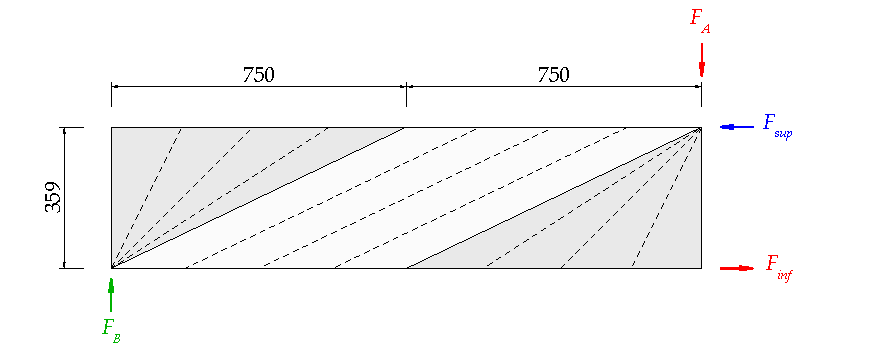
\includegraphics{index_files/mediabag/../imgs/SV14_skd_3.pdf}

}

\caption{\label{fig-skd_3_spannungsfelder_sv14}Schnittkörperdiagramm des
zentrierten Fächers 2}

\end{figure}%

$$
\begin{aligned}
F_{inf_{3}} &= F_{B} \cdot 2 \cdot \frac{ z_{SV14} }{ \tan \left( \theta_{c3_{SV14}} \right) } \cdot \frac{1} { z_{SV14} } \; 
\end{aligned}
$$

$$
\begin{aligned}
F_{inf_{3}} &= 438.7\ \mathrm{kN} \;
\end{aligned}
$$

$$
\begin{aligned}
F_{sup_{3}} &= F_{inf_{3}} \; 
\end{aligned}
$$

$$
\begin{aligned}
F_{sup_{3}} &= 438.7\ \mathrm{kN} \;
\end{aligned}
$$

\begin{figure}[H]

\centering{

\includegraphics{index_files/mediabag/05_Versuchsnachrechnung_VM1_files/figure-pdf/fig-gurtkraft_sv14-output-1.pdf}

}

\caption{\label{fig-gurtkraft_sv14}Gurtkraftverläufe bestimmt anhand der
Spannungsfelder in Abbildung~\ref{fig-spannungsfelder_sv14}. Dargestellt
ist der gesamte Gurtkraftverlauf, sowie der Anteil aus dem Biegemoment}

\end{figure}%

Wird der Anteil des Biegemoments am Gurtkraftverlauf subtrahiert und mit
dem Hebelarm der inneren Kräfte multipliziert, so resultiert das
Versatzmoment.

\[
\Delta_F = F_{inf} - F_M
\] \[
\Delta_M = \Delta_F \cdot z
\]

\begin{figure}[H]

\centering{

\includegraphics{index_files/mediabag/05_Versuchsnachrechnung_VM1_files/figure-pdf/fig-versatzmoment_sv14-output-1.pdf}

}

\caption{\label{fig-versatzmoment_sv14}Versatzmoment dargestellt entlang
der Stabachse}

\end{figure}%

\subsection{Wegfedercharakteristik}\label{wegfedercharakteristik-1}

\subsubsection{Schiebung}\label{schiebung-1}

Die Wegfedercharakteristik basiert auf der Spannungsfeldmodellierung
gemäss der Abbildung~\ref{fig-spannungsfelder_sv14}. Die Einteilung in
Spannungsfelder ermöglicht die Bestimmung der mitwirkenden
Schubbewehrung beim Versagen des Querschnitts. Die Neigung des Feldes
ist so gewählt damit der Querkraftwiderstand der Schubbewehrung der
Traglast des Systems entspricht.

\begin{figure}[H]

\centering{

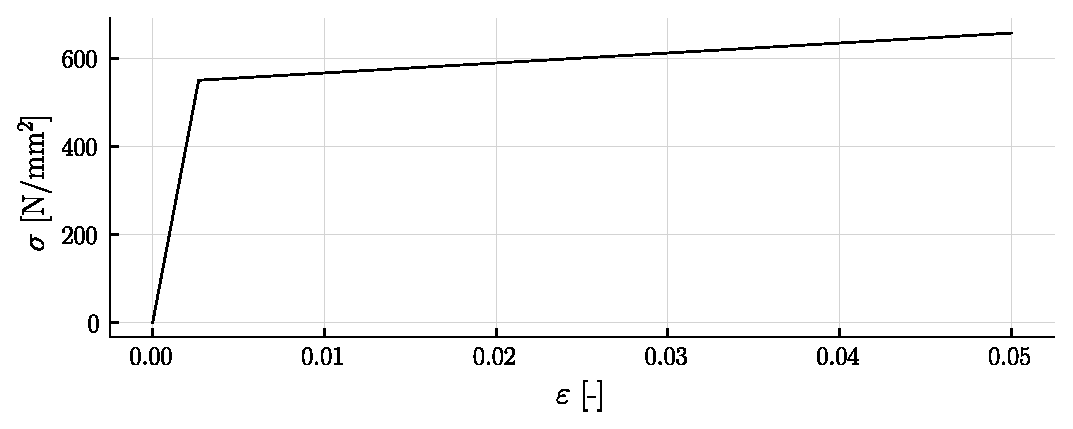
\includegraphics{index_files/mediabag/05_Versuchsnachrechnung_VM1_files/figure-pdf/fig-sigma-epsilon-sv14-output-1.pdf}

}

\caption{\label{fig-sigma-epsilon-sv14}Spannungs-Dehnungs-Beziehung der
Schubbewehrung, übernommen aus
{[}\citeproc{ref-gitz_ansatze_2024}{1}{]}}

\end{figure}%

Folgend sind die Parameter zur Bestimmung der Wegfedercharakteristik in
vertikaler Richtung gezeigt.

$$
\begin{aligned}
E_{sw_{SV14}} &= 205000.0\ \frac{\mathrm{N}}{\mathrm{mm}^{2}} \; 
 &E_{sh_{SV14}} &= 3487.1\ \frac{\mathrm{N}}{\mathrm{mm}^{2}} \;
\end{aligned}
$$

Die Querschnittsfläche der Schubbewehrung und der Bewehrungsgehalt
bestimmt sich zu:

$$
\begin{aligned}
\rho_{sw_{SV14}} &= \frac{ a_{sw_{SV14}} }{ b_{w_{SV14}} } \; 
\end{aligned}
$$

$$
\begin{aligned}
\rho_{sw_{SV14}} &= 0.11\ \mathrm{\%} \;
\end{aligned}
$$

Der Reduktionsfaktor bestimmt sich zu:

$$
\begin{aligned}
\gamma_{E_{SV14}} &= z_{SV14} \cdot \frac{ 1 }{ \tan \left( \theta_{c3_{SV14}} \right) } \cdot \frac{1} { l_{E} } \; 
\end{aligned}
$$

$$
\begin{aligned}
\gamma_{E_{SV14}} &= 75\ \;
\end{aligned}
$$

Die Abbildung~\ref{fig-wegfeder-schub-sv14} zeigt das
Kraft-Verformungs-Verhalten für die Gelenke des Stabmodells in
vertikaler Richtung.

\begin{figure}[H]

\centering{

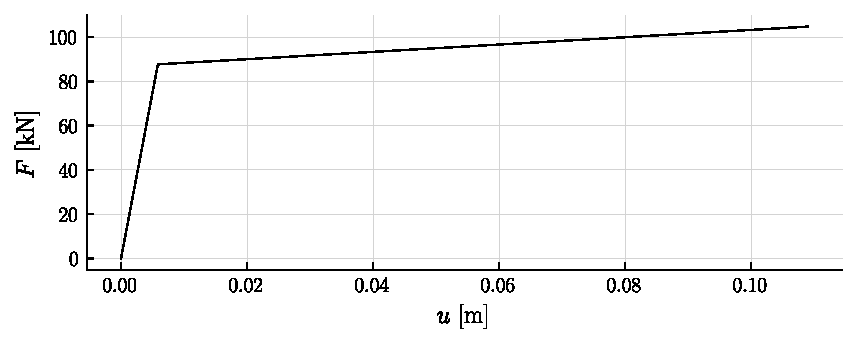
\includegraphics{index_files/mediabag/05_Versuchsnachrechnung_VM1_files/figure-pdf/fig-wegfeder-schub-sv14-output-1.pdf}

}

\caption{\label{fig-wegfeder-schub-sv14}Berechnete
Wegfedercharakteristik des Schubgelenks vom Versuch SV14}

\end{figure}%

\subsection{Versuchsvergleich}\label{versuchsvergleich-1}

Mit den bestimmten Federcharakteristiken kann die Biegelinie des Systems
ermittelt werden unter Berücksichtigung der Schub- und Biegeverformungen
auf nicht-linearen Grundlagen. Die Abbildung~\ref{fig-l-w-sv14} zeigt
das Last-Verformungs-Diagramm des Systems am Punkt \(w_1\). Der
Verformungsverlauf zeigt Abweichungen zu den gemessenen Resultate. Dies
ist auf das Unterschlagen der Längszugkraft aus Querkraft
zurückzuführen.

\begin{figure}[H]

\centering{

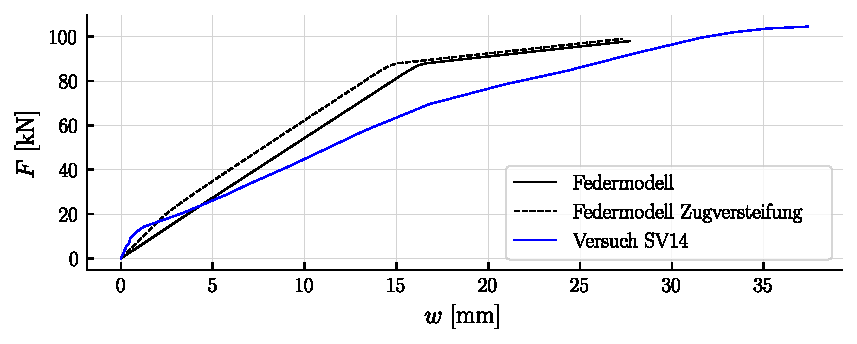
\includegraphics{index_files/mediabag/05_Versuchsnachrechnung_VM1_files/figure-pdf/fig-l-w-sv14-output-1.pdf}

}

\caption{\label{fig-l-w-sv14}Last-Verformungs-Verlauf am Punkt \(w_1\),
für das Federmodell und den Versuch}

\end{figure}%

\bookmarksetup{startatroot}

\chapter{Vorgespannter Träger}\label{vorgespannter-truxe4ger}

Die folgende Versuchsnachrechnung zeigt die Möglichkeiten des Modells im
Bezug mit einer Vorspannung.

\section{Versuchsbeschrieb}\label{versuchsbeschrieb}

In diesem Kapitel wird der vorgespannte Träger T6 nach dem
Versuchsbericht {[}\citeproc{ref-sigrist_versuche_1993}{5}{]} mit dem
Drehfedermodell nachgerechnet. Es handelt sich um einen einfachen Balken
mit einer Auskragung. Die Geometrie des Versuchs in Längsrichtung ist in
Abbildung~\ref{fig-geometrie_t6} gezeigt.

\begin{figure}[H]

\centering{

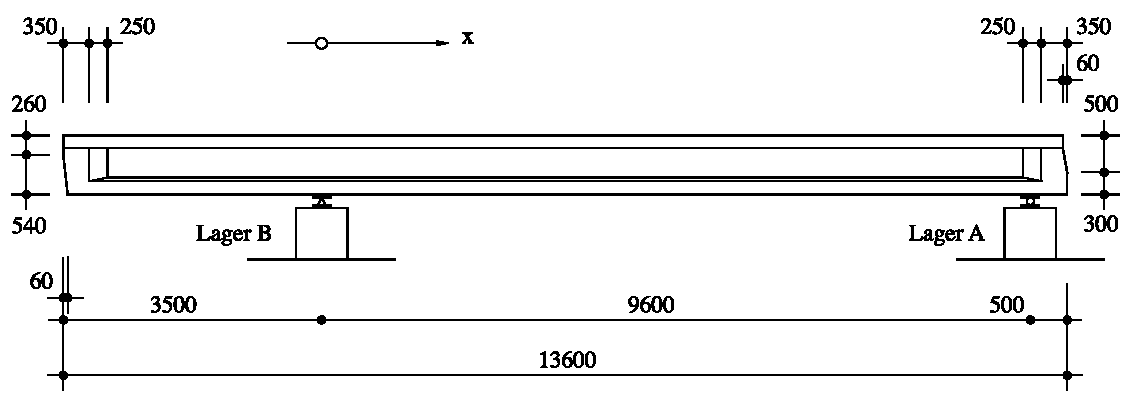
\includegraphics{index_files/mediabag/../imgs/T6_geometrie_laengs.pdf}

}

\caption{\label{fig-geometrie_t6}Geometrie des Versuchsträgers T6,
entnommen aus {[}\citeproc{ref-sigrist_versuche_1993}{5}{]}}

\end{figure}%

Der dazugehörige Querschnitt ist in Abbildung~\ref{fig-geometrie_qs_t6}
gezeigt.

\begin{figure}[H]

\centering{

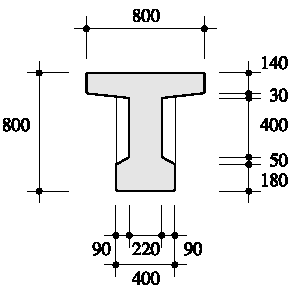
\includegraphics{index_files/mediabag/../imgs/T6_geometrie_qs.pdf}

}

\caption{\label{fig-geometrie_qs_t6}Geometrie des Querschnitts des
Versuchsträgers T6, entnommen aus
{[}\citeproc{ref-sigrist_versuche_1993}{5}{]}}

\end{figure}%

Die Lastsituation zeigt die Abbildung~\ref{fig-last_t6}. Am Ende des
Kragarms greift eine Einzellast \(P\) an. Mit \(Q\) wird eine
Streckenlast simuliert. Der Träger ist an den Punkten \(A\) und \(B\)
einfach gelagert.

\begin{figure}[H]

\centering{

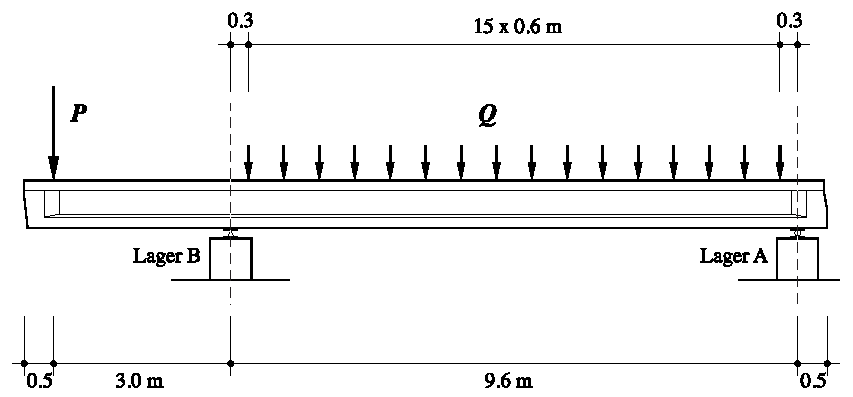
\includegraphics{index_files/mediabag/../imgs/T6_last_laengs.pdf}

}

\caption{\label{fig-last_t6}Lagerung und Laststellung des
Versuchsträgers T6, entnommen aus
{[}\citeproc{ref-sigrist_versuche_1993}{5}{]}}

\end{figure}%

Die verlegte schlaffe Bewehrung in Längsrichtung ist in der
Abbildung~\ref{fig-bewehrung_laengs_t6} gezeigt.

\begin{figure}[H]

\centering{

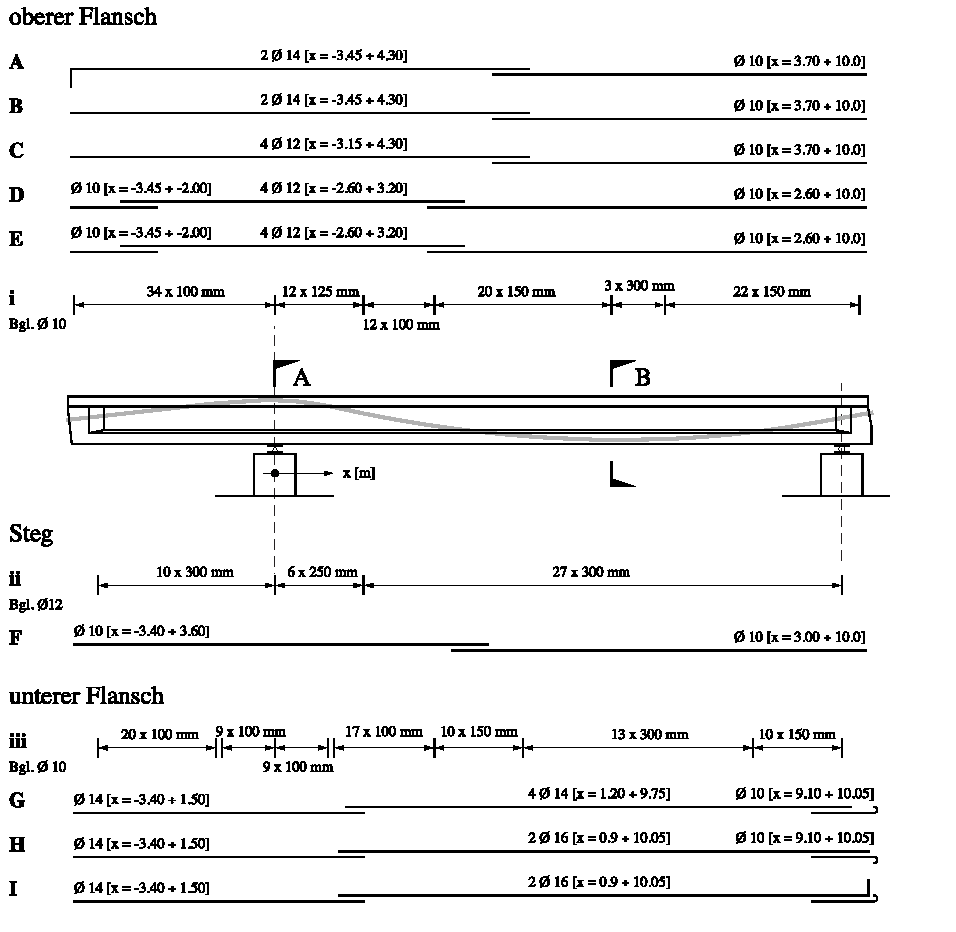
\includegraphics{index_files/mediabag/../imgs/T6_bewehrung_laengs.pdf}

}

\caption{\label{fig-bewehrung_laengs_t6}Bewehrungslayout in
Längsrichtung des Versuchsträgers T6, entnommen aus
{[}\citeproc{ref-sigrist_versuche_1993}{5}{]}}

\end{figure}%

Das Bewehrungslayout im Querschnitt zeigt die
Abbildung~\ref{fig-bewehrung_qs_t6}.

\begin{figure}[H]

\centering{

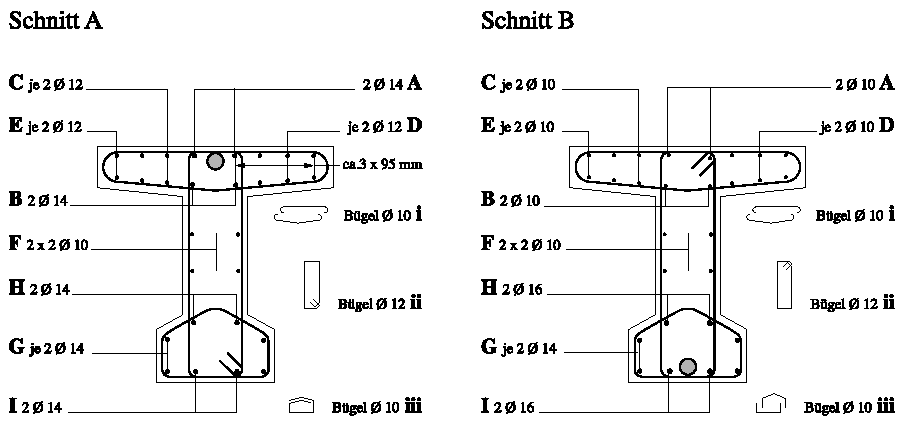
\includegraphics{index_files/mediabag/../imgs/T6_bewehrung_qs.pdf}

}

\caption{\label{fig-bewehrung_qs_t6}Bewehrungslayout im Querschnitt des
Versuchsträgers T6, entnommen aus
{[}\citeproc{ref-sigrist_versuche_1993}{5}{]}}

\end{figure}%

Die Führung der Vorspannung ist in der
Abbildung~\ref{fig-vorspannung_t6} gezeigt.

\begin{figure}[H]

\centering{

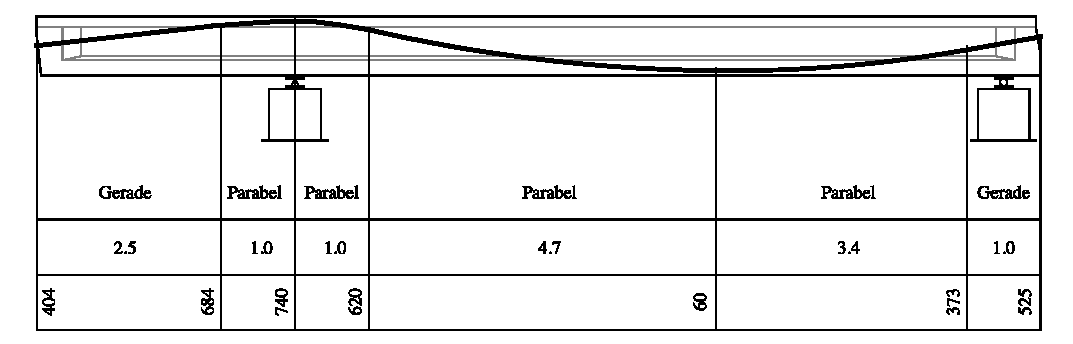
\includegraphics{index_files/mediabag/../imgs/T6_vorspannung_laengs.pdf}

}

\caption{\label{fig-vorspannung_t6}Vorspannungslayout des
Versuchsträgers T6. Horizontaler Abstand {[}m{]} und vertikale Position
{[}mm{]}, gemessen von der Unterkante des Trägers, entnommen aus
{[}\citeproc{ref-sigrist_versuche_1993}{5}{]}}

\end{figure}%

\section{Parameter}\label{parameter}

In diesem Abschnitt werden die allgemein verwendeten Parameter
aufgelistet. Gegliedert nach den einzelnen Aspekten des Versuchs.

\subsection{Vorspannung}\label{vorspannung}

Die Parameter der Vorspannung sind die Folgenden. Es ist die Initiale
Vorspannkraft, sowie die entsprechenden Querschnittseigenschaften
aufgezeigt:

$$
\begin{aligned}
f_{py} &= 1706.0\ \frac{\mathrm{N}}{\mathrm{mm}^{2}} \; 
 &f_{pt} &= 1855.0\ \frac{\mathrm{N}}{\mathrm{mm}^{2}} \; 
 &V_{om} &= 730.0\ \mathrm{kN} \; 
\\[11pt]
 A_{p} &= 596.0\ \mathrm{mm}^{2} \; 
 &E_{p} &= 190000.0\ \frac{\mathrm{N}}{\mathrm{mm}^{2}} \; 
 &\varepsilon_{pu} &= 1.5\ \mathrm{\%} \; 
\\[11pt]
 \eta &= 0.9 \; \;\textrm{(Verlustfaktor)}
\end{aligned}
$$

Der Verlustfaktor wird ohne Berücksichtigung von Langzeiteffekten auf
90\% geschätzt. Daras resultiert die Vorspannkraft zu:

$$
\begin{aligned}
P_{\infty} &= \eta \cdot V_{om} \; 
\end{aligned}
$$

$$
\begin{aligned}
P_{\infty} &= 657.0\ \mathrm{kN} \;
\end{aligned}
$$

Die Spannung im Spannstahl:

$$
\begin{aligned}
\sigma_{P_{\infty}} &= \frac{ P_{\infty} }{ A_{p} } \; 
\end{aligned}
$$

$$
\begin{aligned}
\sigma_{P_{\infty}} &= 1102.3\ \frac{\mathrm{N}}{\mathrm{mm}^{2}} \;
\end{aligned}
$$

\includegraphics{index_files/mediabag/06_Vorspannversuch_files/figure-pdf/cell-8-output-1.pdf}

\subsection{Beton}\label{beton}

Die Parameter sind Mittelwerte aus Betonwürfel- und Betonzylinderproben.

$$
\begin{aligned}
f_{c} &= 52.10\ \frac{\mathrm{N}}{\mathrm{mm}^{2}} \; 
 &f_{cts} &= 4.30\ \frac{\mathrm{N}}{\mathrm{mm}^{2}} \; 
 &E_{c} &= 50200.00\ \frac{\mathrm{N}}{\mathrm{mm}^{2}} \; 
\\[11pt]
 \rho_{c} &= 2409.00\ \frac{\mathrm{kg}}{\mathrm{m}^{3}} \; 
 &\varepsilon_{cu} &= 0.16\ \mathrm{\%} \;
\end{aligned}
$$

Das Spannungs-Dehnungs-Verhalten des Betons ist in der
Abbildung~\ref{fig-sigma_epc_t6} dargestellt. Definiert ist das
Verhalten im positiven Spannungsbereich bis zum Erreichen der
Betonzugfestigkeit \(f_{cts}\). Das Verhalten im negativen
Spannungsbereich wird mit einem linear-elastischem ideal-plastischem
Verhalten approximiert.

\subsection{Betonstahl}\label{betonstahl}

Mittelwerte der Zugproben.

$$
\begin{aligned}
\oslash_{1} &= 10.0\ \mathrm{mm} \; 
 &\oslash_{2} &= 12.0\ \mathrm{mm} \; 
 &\oslash_{3} &= 14.0\ \mathrm{mm} \; 
\\[11pt]
 f_{sy} &= 500.0\ \mathrm{MPa} \; 
 &f_{st} &= 630.0\ \mathrm{MPa} \; 
 &\varepsilon_{sv} &= 2.4\ \mathrm{\%} \; 
\\[11pt]
 E_{s} &= 205000.0\ \frac{\mathrm{N}}{\mathrm{mm}^{2}} \;
\end{aligned}
$$

Die entsprechende Spannungs-Dehnungs-Beziehung ist in
Abbildung~\ref{fig-sigma_eps_t6} gezeigt. Als Annahme gilt, dass die
Stäbe lediglich unter Zug belastet werden. Die Druckbewehrung wird bei
der Bestimmung der Momenten-Krümmungs-Beziehung vernachlässigt. Das
Verhalten wird mit einem Bilinearem Verhalten approximiert.

\subsection{Geometrie}\label{geometrie}

\subsubsection{Querschnitt}\label{querschnitt}

Die Parameter der Geometrie des Querschnitts beziehen sich auf die
Abbildung~\ref{fig-geometrie_qs_t6}.

$$
\begin{aligned}
h_{1} &= 180.0\ \mathrm{mm} \; 
 &h_{2} &= 50.0\ \mathrm{mm} \; 
 &h_{3} &= 400.0\ \mathrm{mm} \; 
\\[11pt]
 h_{4} &= 30.0\ \mathrm{mm} \; 
 &h_{5} &= 140.0\ \mathrm{mm} \; 
 &h_{tot} &= 800.0\ \mathrm{mm} \; 
\\[11pt]
 b_{1_{inf}} &= 90.0\ \mathrm{mm} \; 
 &b_{2_{inf}} &= 220.0\ \mathrm{mm} \; 
 &b_{3_{inf}} &= 90.0\ \mathrm{mm} \; 
\\[11pt]
 b_{tot_{inf}} &= 400.0\ \mathrm{mm} \; 
 &b_{tot_{sup}} &= 800.0\ \mathrm{mm} \; 
 &S_{z} &= \mathtt{\text{464.00 mm}} \; 
\\[11pt]
\end{aligned}
$$

Schwerpunkt des Querschnitts von der Unterkante aus gemessen:

\subsubsection{Längsrichtung}\label{luxe4ngsrichtung}

Der Abschluss des Querschnitts wird nicht mehr weiter verfolgt.
Vereinfacht wird der I-Querschnitt als konstant über die Länge
betrachtet.

Die beschriebenen Abmessungen \(L_n\) sind jeweils vom Stabanfang
gemessen.

$$
\begin{aligned}
L_{1} &= 3500.0\ \mathrm{mm} \; 
 &L_{2} &= 9600.0\ \mathrm{mm} \; 
 &L_{3} &= 500.0\ \mathrm{mm} \; 
\\[11pt]
 L_{tot} &= 13600.0\ \mathrm{mm} \;
\end{aligned}
$$

\subsubsection{Lasten}\label{lasten}

$$
\begin{aligned}
L_{P} &= 0.5\ \mathrm{m} \; 
 &L_{q} &= 3.8\ \mathrm{m} \; 
 &l_{q} &= 9.0\ \mathrm{m} \; \;\textrm{(Streckenlast)}
\\[11pt]
\end{aligned}
$$

\section{Modellierung}\label{modellierung}

$$
\begin{aligned}
l_{E} &= 10.0\ \mathrm{cm} \;
\end{aligned}
$$

\subsection{Lastfälle}\label{lastfuxe4lle}

\subsubsection{Versuch}\label{versuch}

Der Versuch wird in den folgenden Laststufen belastet.

$$
\begin{aligned}
Q_{max} &= 1638.0\ \mathrm{kN} \; 
 &P_{max} &= 512.0\ \mathrm{kN} \;
\end{aligned}
$$

$$
\begin{aligned}
q_{Q} &= \frac{ Q_{max} }{ l_{q} }  = \frac{ 1638.0\ \mathrm{kN} }{ 9.0\ \mathrm{m} } &= 182.0\ \frac{\mathrm{kN}}{\mathrm{m}}  
\end{aligned}
$$

\subsubsection{Vorspannung}\label{vorspannung-1}

\includegraphics{index_files/mediabag/06_Vorspannversuch_files/figure-pdf/cell-20-output-1.pdf}

\[
u_p(x) \simeq z_p(x)'' \cdot P
\]

Dies führt zu den Umlenkkräften:

\begin{figure}[H]

\centering{

\includegraphics{index_files/mediabag/06_Vorspannversuch_files/figure-pdf/fig-u_p_von_x-output-1.pdf}

}

\caption{\label{fig-u_p_von_x}Umlenkkräfte ermittelt mit \(z_p(x)''\)}

\end{figure}%

Zusätzlich zu den Umlenkkräften ist bei der Spannstelle eine Druckkraft
in Richtung des Spannkabels einzuführen, sowie ein Versatz Moment, durch
die Exzentrizität des Spannkabels zum Trägerschwerpunkt.

\includegraphics{index_files/mediabag/06_Vorspannversuch_files/figure-pdf/cell-22-output-1.pdf}

$$
\begin{aligned}
e_{P_{0}} &= 60.0\ \mathrm{mm} \; \;\textrm{($x=0$)}
 &e_{P_{1}} &= -60.9\ \mathrm{mm} \; \;\textrm{($x=L_{tot}$)}
\end{aligned}
$$

$$
\begin{aligned}
M_{P_{0}} &= P_{\infty} \cdot e_{P_{0}} \; 
\end{aligned}
$$

$$
\begin{aligned}
M_{P_{0}} &= 39.4\ \mathrm{kN} \cdot \mathrm{m} \;
\end{aligned}
$$

$$
\begin{aligned}
M_{P_{1}} &= P_{\infty} \cdot e_{P_{1}} \; 
\end{aligned}
$$

$$
\begin{aligned}
M_{P_{1}} &= -40.0\ \mathrm{kN} \cdot \mathrm{m} \;
\end{aligned}
$$

\section{Momenten-Krümmungs-Beziehung}\label{momenten-kruxfcmmungs-beziehung}

Die Momenten-Krümmungs-Beziehung zeigt bei diesem Versuch eine gewisse
Komplexität. Grundsätzlich gilt es für jede Abstufung der Bewehrung eine
separate Momenten-Krümmungs-Beziehung herzuleiten.

Wird bei der Vorspannung Spannkraftverluste berücksichtigt, so wirkt der
Restquerschnitt des Spannstahls als schlaffe Bewehrung bei Belastung
mit. Dies hat Einfluss auf das Momenten-Krümmungs-Verhalten. Durch die
parabolische Geometrie des Spannkabels, gilt es die
Momenten-Krümmungs-Beziehung unter Variation der Spannkabellage zu
definieren, was die Komplexität der Momenten-Krümmungs-Beziehung erhöht.

Um den Rechenaufwand gering zu halten wird lediglich ein qualitatives
Verhalten der Momenten-Krümmungs-Beziehung angestrebt. Dabei wird der
Querschnitt beim Fliessen der Zugbewehrung betrachtet, sowie wird der
Biegewiderstand bestimmt. Diese Punkte werden linear mit einander
verbunden. Des Weiteren wird die Druckbewehrung stehts vernachlässigt.

\begin{figure}[H]

\centering{

\includegraphics{index_files/mediabag/../imgs/QS_14_analyse_4.pdf}

}

\caption{\label{fig-qs_fliessen_qualitativ}Querschnittsanalyse mit
Fliessen der Zugbewehrung und elastischer Betondruckzone, qualitativer
Verlauf}

\end{figure}%

\begin{figure}[H]

\centering{

\includegraphics{index_files/mediabag/../imgs/QS_14_analyse_5.pdf}

}

\caption{\label{fig-qs_widerstand_qualitativ}Querschnittsanalyse mit
erreichter Zugfestigkeit in der Bewehrung und vollständig
plastifizierter Betondruckzone, qualitativer Verlauf}

\end{figure}%

\subsection{Abschätzung}\label{abschuxe4tzung}

Hier wird die Krümmung und das Biegemoment für den Querschnitt A-A
abgeschätzt, als Referenzwerte für die numerisch erstellten
Momenten-Krümmungs-Diagramme.

$$
\begin{aligned}
A_{s_{1}} &= \left( 4 \cdot \frac{ \left( 14 \cdot \mathrm{mm} \right) ^{ 2 } }{ 4 } + 12 \cdot \frac{ \left( 12 \cdot \mathrm{mm} \right) ^{ 2 } }{ 4 } \right) \cdot \pi \; 
\end{aligned}
$$

$$
\begin{aligned}
A_{s_{1}} &= 1972.9\ \mathrm{mm}^{2} \;
\end{aligned}
$$

$$
\begin{aligned}
d_{\sim} &= 750 \cdot \mathrm{mm} \; 
\\[11pt]
z_{\sim} &= 0.9 \cdot d_{\sim} \; 
\end{aligned}
$$

$$
\begin{aligned}
z_{\sim} &= 675.0\ \mathrm{mm} \;
\end{aligned}
$$

$$
\begin{aligned}
x_{\sim} &= \frac{ A_{s_{1}} \cdot f_{st} + A_{p} \cdot \left( f_{pt} - \sigma_{P_{\infty}} \right) }{ b_{tot_{inf}} \cdot 0.85 \cdot f_{c} } \; 
\end{aligned}
$$

$$
\begin{aligned}
x_{\sim} &= 95.5\ \mathrm{mm} \;
\end{aligned}
$$

$$
\begin{aligned}
M_{R_{\sim}} &= z_{\sim} \cdot \left( A_{s_{1}} \cdot f_{sy} + A_{p} \cdot \left( f_{py} - \sigma_{P_{\infty}} \right) \right) \; 
\end{aligned}
$$

$$
\begin{aligned}
M_{R_{\sim}} &= 908.7\ \mathrm{kN} \cdot \mathrm{m} \;
\end{aligned}
$$

$$
\begin{aligned}
\chi_{\sim} &= \frac{ \varepsilon_{sv} }{ d_{\sim} - x_{\sim} } \; 
\end{aligned}
$$

$$
\begin{aligned}
\chi_{\sim} &= 0.0367\ \frac{1}{\mathrm{m}} \;
\end{aligned}
$$

\subsection{Stoffgesetze}\label{stoffgesetze}

\begin{figure}[H]

\centering{

\includegraphics{index_files/mediabag/06_Vorspannversuch_files/figure-pdf/fig-sigma_epc_t6-output-1.pdf}

}

\caption{\label{fig-sigma_epc_t6}Spannungs-Dehnungs-Verhalten des
Betons}

\end{figure}%

\begin{figure}[H]

\centering{

\includegraphics{index_files/mediabag/06_Vorspannversuch_files/figure-pdf/fig-sigma_eps_t6-output-1.pdf}

}

\caption{\label{fig-sigma_eps_t6}Spannungs-Dehnungs-Verhalten des
Betonstahls}

\end{figure}%

Die Spannungs-Dehnungs-Beziehung des Spannstahls wird mit der
Vorspannspannung \(\sigma_{P\infty}\) reduziert.

\begin{figure}[H]

\centering{

\includegraphics{index_files/mediabag/06_Vorspannversuch_files/figure-pdf/fig-sigma_eps_vorspannung_t6-output-1.pdf}

}

\caption{\label{fig-sigma_eps_vorspannung_t6}Spannungs-Dehnungs-Verhalten
der Vorspannung}

\end{figure}%

\section{Schiebungs-Beziehung}\label{schiebungs-beziehung}

\section{Versuchsresultate}\label{versuchsresultate}

\begin{figure}[H]

\centering{

\includegraphics{index_files/mediabag/../imgs/T6_durchbiegung_laengs.pdf}

}

\caption{\label{fig-durchbiegung_laengs_t6}Verformungsverlauf des
Versuchsträgers T6, entnommen aus
{[}\citeproc{ref-sigrist_versuche_1993}{5}{]}}

\end{figure}%

\begin{figure}[H]

\centering{

\includegraphics{index_files/mediabag/../imgs/T6_durchbiegungen.pdf}

}

\caption{\label{fig-durchbiegung_t6}Last-Verformungs-Verhalten des
Versuchsträgers T6, entnommen aus
{[}\citeproc{ref-sigrist_versuche_1993}{5}{]}}

\end{figure}%

\bookmarksetup{startatroot}

\chapter{IdeaStatica}\label{ideastatica}

In diesem Kapitel wird darauf abgezielt, das Verformungsverhalten der
behandelten Versuche mit einer kommerziellen Software zu bestimmen. Das
Ziel ist es die Resultate der Software auf Präzision zu prüfen, sowie
die Eingabe des Modells zu verstehen.

Dabei wird die Modellaufbereitung beschrieben, sowie einzelne
Eingabeparameter diskutiert.

\bookmarksetup{startatroot}

\chapter*{Literatur}\label{literatur}
\addcontentsline{toc}{chapter}{Literatur}

\markboth{Literatur}{Literatur}

\phantomsection\label{refs}
\begin{CSLReferences}{0}{1}
\bibitem[\citeproctext]{ref-gitz_ansatze_2024}
\CSLLeftMargin{1. }%
\CSLRightInline{Gitz P (2024) Ansätze zur {Verformungsberechnung}. HSLU
Technik \& Architektur}

\bibitem[\citeproctext]{ref-jager_versuche_2006}
\CSLLeftMargin{2. }%
\CSLRightInline{Jäger T, Marti P (2006) Versuche zum
{Querkraftwiderstand} und zum {Verformungsvermögen} von
{Stahlbetonplatten}. IBK Bericht 294.
\url{https://doi.org/10.3929/ethz-a-005195576}}

\bibitem[\citeproctext]{ref-tue_einfluss_2019}
\CSLLeftMargin{3. }%
\CSLRightInline{Tue NV, Ehmann R, Betschoga C, Tung ND (2019) Einfluss
geringer {Querkraftbewehrung} auf die {Querkrafttragfähigkeit} von
{Stahlbetonbalken} unterschiedlicher {M}/{V}-{Kombinationen}. Beton- und
Stahlbetonbau 114(4):217--230.
https://doi.org/\url{https://doi.org/10.1002/best.201800075}}

\bibitem[\citeproctext]{ref-marienhutte_produktdatenblatt_b550bpdf_nodate}
\CSLLeftMargin{4. }%
\CSLRightInline{Marienhütte
\href{https://www.marienhuette.at/wp-content/uploads/Produktdatenblatt-B550B.pdf}{Produktdatenblatt\_B550B.pdf}}

\bibitem[\citeproctext]{ref-sigrist_versuche_1993}
\CSLLeftMargin{5. }%
\CSLRightInline{Sigrist V, Marti P (1993) Versuche zum
{Verformungsvermögen} von {Stahlbetonträgern}. Birkhäuser, Basel Boston
Berlin}

\end{CSLReferences}

\cleardoublepage
\phantomsection
\addcontentsline{toc}{part}{Anhang}
\appendix

\chapter{Momenten-Krümmungs-Beziehungen Versuch
T6}\label{momenten-kruxfcmmungs-beziehungen-versuch-t6}

Dieses Kapitel zeigt lediglich die einzelnen Querschnitte mit den
entsprechenden Parametern und der resultierenden
Momenten-Krümmungs-Beziehung. Es wird keinen Wert auf die Leserlichkeit
in Papierformat gelegt.

\begin{figure}[H]

{\centering \includegraphics{index_files/mediabag/T6_m_chi/m_chi_tot.pdf}

}

\caption{Überlagerung der einzelnen Momenten-Krümmungs-Beziehungen}

\end{figure}%

\begin{figure}[H]

\begin{minipage}{0.50\linewidth}
\includegraphics{index_files/mediabag/T6_m_chi/qs_0.pdf}\end{minipage}%
%
\begin{minipage}{0.50\linewidth}
\includegraphics{index_files/mediabag/T6_m_chi/m_chi_0.pdf}\end{minipage}%

\caption{\label{fig-m_chi_appendix}Momenten-Krümmungs-Beziehung des
Querschnitts 0}

\end{figure}%

\begin{figure}[H]

\begin{minipage}{0.50\linewidth}
\includegraphics{index_files/mediabag/T6_m_chi/qs_1.pdf}\end{minipage}%
%
\begin{minipage}{0.50\linewidth}
\includegraphics{index_files/mediabag/T6_m_chi/m_chi_1.pdf}\end{minipage}%

\caption{\label{fig-m_chi_appendix}Momenten-Krümmungs-Beziehung des
Querschnitts 1}

\end{figure}%

\begin{figure}[H]

\begin{minipage}{0.50\linewidth}
\includegraphics{index_files/mediabag/T6_m_chi/qs_2.pdf}\end{minipage}%
%
\begin{minipage}{0.50\linewidth}
\includegraphics{index_files/mediabag/T6_m_chi/m_chi_2.pdf}\end{minipage}%

\caption{\label{fig-m_chi_appendix}Momenten-Krümmungs-Beziehung des
Querschnitts 2}

\end{figure}%

\begin{figure}[H]

\begin{minipage}{0.50\linewidth}
\includegraphics{index_files/mediabag/T6_m_chi/qs_3.pdf}\end{minipage}%
%
\begin{minipage}{0.50\linewidth}
\includegraphics{index_files/mediabag/T6_m_chi/m_chi_3.pdf}\end{minipage}%

\caption{\label{fig-m_chi_appendix}Momenten-Krümmungs-Beziehung des
Querschnitts 3}

\end{figure}%

\begin{figure}[H]

\begin{minipage}{0.50\linewidth}
\includegraphics{index_files/mediabag/T6_m_chi/qs_4.pdf}\end{minipage}%
%
\begin{minipage}{0.50\linewidth}
\includegraphics{index_files/mediabag/T6_m_chi/m_chi_4.pdf}\end{minipage}%

\caption{\label{fig-m_chi_appendix}Momenten-Krümmungs-Beziehung des
Querschnitts 4}

\end{figure}%

\begin{figure}[H]

\begin{minipage}{0.50\linewidth}
\includegraphics{index_files/mediabag/T6_m_chi/qs_5.pdf}\end{minipage}%
%
\begin{minipage}{0.50\linewidth}
\includegraphics{index_files/mediabag/T6_m_chi/m_chi_5.pdf}\end{minipage}%

\caption{\label{fig-m_chi_appendix}Momenten-Krümmungs-Beziehung des
Querschnitts 5}

\end{figure}%

\begin{figure}[H]

\begin{minipage}{0.50\linewidth}
\includegraphics{index_files/mediabag/T6_m_chi/qs_6.pdf}\end{minipage}%
%
\begin{minipage}{0.50\linewidth}
\includegraphics{index_files/mediabag/T6_m_chi/m_chi_6.pdf}\end{minipage}%

\caption{\label{fig-m_chi_appendix}Momenten-Krümmungs-Beziehung des
Querschnitts 6}

\end{figure}%

\begin{figure}[H]

\begin{minipage}{0.50\linewidth}
\includegraphics{index_files/mediabag/T6_m_chi/qs_7.pdf}\end{minipage}%
%
\begin{minipage}{0.50\linewidth}
\includegraphics{index_files/mediabag/T6_m_chi/m_chi_7.pdf}\end{minipage}%

\caption{\label{fig-m_chi_appendix}Momenten-Krümmungs-Beziehung des
Querschnitts 7}

\end{figure}%

\begin{figure}[H]

\begin{minipage}{0.50\linewidth}
\includegraphics{index_files/mediabag/T6_m_chi/qs_8.pdf}\end{minipage}%
%
\begin{minipage}{0.50\linewidth}
\includegraphics{index_files/mediabag/T6_m_chi/m_chi_8.pdf}\end{minipage}%

\caption{\label{fig-m_chi_appendix}Momenten-Krümmungs-Beziehung des
Querschnitts 8}

\end{figure}%

\begin{figure}[H]

\begin{minipage}{0.50\linewidth}
\includegraphics{index_files/mediabag/T6_m_chi/qs_9.pdf}\end{minipage}%
%
\begin{minipage}{0.50\linewidth}
\includegraphics{index_files/mediabag/T6_m_chi/m_chi_9.pdf}\end{minipage}%

\caption{\label{fig-m_chi_appendix}Momenten-Krümmungs-Beziehung des
Querschnitts 9}

\end{figure}%

\begin{figure}[H]

\begin{minipage}{0.50\linewidth}
\includegraphics{index_files/mediabag/T6_m_chi/qs_10.pdf}\end{minipage}%
%
\begin{minipage}{0.50\linewidth}
\includegraphics{index_files/mediabag/T6_m_chi/m_chi_10.pdf}\end{minipage}%

\caption{\label{fig-m_chi_appendix}Momenten-Krümmungs-Beziehung des
Querschnitts 10}

\end{figure}%

\begin{figure}[H]

\begin{minipage}{0.50\linewidth}
\includegraphics{index_files/mediabag/T6_m_chi/qs_11.pdf}\end{minipage}%
%
\begin{minipage}{0.50\linewidth}
\includegraphics{index_files/mediabag/T6_m_chi/m_chi_11.pdf}\end{minipage}%

\caption{\label{fig-m_chi_appendix}Momenten-Krümmungs-Beziehung des
Querschnitts 11}

\end{figure}%

\begin{figure}[H]

\begin{minipage}{0.50\linewidth}
\includegraphics{index_files/mediabag/T6_m_chi/qs_12.pdf}\end{minipage}%
%
\begin{minipage}{0.50\linewidth}
\includegraphics{index_files/mediabag/T6_m_chi/m_chi_12.pdf}\end{minipage}%

\caption{\label{fig-m_chi_appendix}Momenten-Krümmungs-Beziehung des
Querschnitts 12}

\end{figure}%

\begin{figure}[H]

\begin{minipage}{0.50\linewidth}
\includegraphics{index_files/mediabag/T6_m_chi/qs_13.pdf}\end{minipage}%
%
\begin{minipage}{0.50\linewidth}
\includegraphics{index_files/mediabag/T6_m_chi/m_chi_13.pdf}\end{minipage}%

\caption{\label{fig-m_chi_appendix}Momenten-Krümmungs-Beziehung des
Querschnitts 13}

\end{figure}%

\begin{figure}[H]

\begin{minipage}{0.50\linewidth}
\includegraphics{index_files/mediabag/T6_m_chi/qs_14.pdf}\end{minipage}%
%
\begin{minipage}{0.50\linewidth}
\includegraphics{index_files/mediabag/T6_m_chi/m_chi_14.pdf}\end{minipage}%

\caption{\label{fig-m_chi_appendix}Momenten-Krümmungs-Beziehung des
Querschnitts 14}

\end{figure}%

\begin{figure}[H]

\begin{minipage}{0.50\linewidth}
\includegraphics{index_files/mediabag/T6_m_chi/qs_15.pdf}\end{minipage}%
%
\begin{minipage}{0.50\linewidth}
\includegraphics{index_files/mediabag/T6_m_chi/m_chi_15.pdf}\end{minipage}%

\caption{\label{fig-m_chi_appendix}Momenten-Krümmungs-Beziehung des
Querschnitts 15}

\end{figure}%

\begin{figure}[H]

\begin{minipage}{0.50\linewidth}
\includegraphics{index_files/mediabag/T6_m_chi/qs_16.pdf}\end{minipage}%
%
\begin{minipage}{0.50\linewidth}
\includegraphics{index_files/mediabag/T6_m_chi/m_chi_16.pdf}\end{minipage}%

\caption{\label{fig-m_chi_appendix}Momenten-Krümmungs-Beziehung des
Querschnitts 16}

\end{figure}%

\begin{figure}[H]

\begin{minipage}{0.50\linewidth}
\includegraphics{index_files/mediabag/T6_m_chi/qs_17.pdf}\end{minipage}%
%
\begin{minipage}{0.50\linewidth}
\includegraphics{index_files/mediabag/T6_m_chi/m_chi_17.pdf}\end{minipage}%

\caption{\label{fig-m_chi_appendix}Momenten-Krümmungs-Beziehung des
Querschnitts 17}

\end{figure}%

\begin{figure}[H]

\begin{minipage}{0.50\linewidth}
\includegraphics{index_files/mediabag/T6_m_chi/qs_18.pdf}\end{minipage}%
%
\begin{minipage}{0.50\linewidth}
\includegraphics{index_files/mediabag/T6_m_chi/m_chi_18.pdf}\end{minipage}%

\caption{\label{fig-m_chi_appendix}Momenten-Krümmungs-Beziehung des
Querschnitts 18}

\end{figure}%

\begin{figure}[H]

\begin{minipage}{0.50\linewidth}
\includegraphics{index_files/mediabag/T6_m_chi/qs_19.pdf}\end{minipage}%
%
\begin{minipage}{0.50\linewidth}
\includegraphics{index_files/mediabag/T6_m_chi/m_chi_19.pdf}\end{minipage}%

\caption{\label{fig-m_chi_appendix}Momenten-Krümmungs-Beziehung des
Querschnitts 19}

\end{figure}%

\begin{figure}[H]

\begin{minipage}{0.50\linewidth}
\includegraphics{index_files/mediabag/T6_m_chi/qs_20.pdf}\end{minipage}%
%
\begin{minipage}{0.50\linewidth}
\includegraphics{index_files/mediabag/T6_m_chi/m_chi_20.pdf}\end{minipage}%

\caption{\label{fig-m_chi_appendix}Momenten-Krümmungs-Beziehung des
Querschnitts 20}

\end{figure}%

\begin{figure}[H]

\begin{minipage}{0.50\linewidth}
\includegraphics{index_files/mediabag/T6_m_chi/qs_21.pdf}\end{minipage}%
%
\begin{minipage}{0.50\linewidth}
\includegraphics{index_files/mediabag/T6_m_chi/m_chi_21.pdf}\end{minipage}%

\caption{\label{fig-m_chi_appendix}Momenten-Krümmungs-Beziehung des
Querschnitts 21}

\end{figure}%

\begin{figure}[H]

\begin{minipage}{0.50\linewidth}
\includegraphics{index_files/mediabag/T6_m_chi/qs_22.pdf}\end{minipage}%
%
\begin{minipage}{0.50\linewidth}
\includegraphics{index_files/mediabag/T6_m_chi/m_chi_22.pdf}\end{minipage}%

\caption{\label{fig-m_chi_appendix}Momenten-Krümmungs-Beziehung des
Querschnitts 22}

\end{figure}%

\begin{figure}[H]

\begin{minipage}{0.50\linewidth}
\includegraphics{index_files/mediabag/T6_m_chi/qs_23.pdf}\end{minipage}%
%
\begin{minipage}{0.50\linewidth}
\includegraphics{index_files/mediabag/T6_m_chi/m_chi_23.pdf}\end{minipage}%

\caption{\label{fig-m_chi_appendix}Momenten-Krümmungs-Beziehung des
Querschnitts 23}

\end{figure}%

\begin{figure}[H]

\begin{minipage}{0.50\linewidth}
\includegraphics{index_files/mediabag/T6_m_chi/qs_24.pdf}\end{minipage}%
%
\begin{minipage}{0.50\linewidth}
\includegraphics{index_files/mediabag/T6_m_chi/m_chi_24.pdf}\end{minipage}%

\caption{\label{fig-m_chi_appendix}Momenten-Krümmungs-Beziehung des
Querschnitts 24}

\end{figure}%

\begin{figure}[H]

\begin{minipage}{0.50\linewidth}
\includegraphics{index_files/mediabag/T6_m_chi/qs_25.pdf}\end{minipage}%
%
\begin{minipage}{0.50\linewidth}
\includegraphics{index_files/mediabag/T6_m_chi/m_chi_25.pdf}\end{minipage}%

\caption{\label{fig-m_chi_appendix}Momenten-Krümmungs-Beziehung des
Querschnitts 25}

\end{figure}%

\begin{figure}[H]

\begin{minipage}{0.50\linewidth}
\includegraphics{index_files/mediabag/T6_m_chi/qs_26.pdf}\end{minipage}%
%
\begin{minipage}{0.50\linewidth}
\includegraphics{index_files/mediabag/T6_m_chi/m_chi_26.pdf}\end{minipage}%

\caption{\label{fig-m_chi_appendix}Momenten-Krümmungs-Beziehung des
Querschnitts 26}

\end{figure}%

\begin{figure}[H]

\begin{minipage}{0.50\linewidth}
\includegraphics{index_files/mediabag/T6_m_chi/qs_27.pdf}\end{minipage}%
%
\begin{minipage}{0.50\linewidth}
\includegraphics{index_files/mediabag/T6_m_chi/m_chi_27.pdf}\end{minipage}%

\caption{\label{fig-m_chi_appendix}Momenten-Krümmungs-Beziehung des
Querschnitts 27}

\end{figure}%

\begin{figure}[H]

\begin{minipage}{0.50\linewidth}
\includegraphics{index_files/mediabag/T6_m_chi/qs_28.pdf}\end{minipage}%
%
\begin{minipage}{0.50\linewidth}
\includegraphics{index_files/mediabag/T6_m_chi/m_chi_28.pdf}\end{minipage}%

\caption{\label{fig-m_chi_appendix}Momenten-Krümmungs-Beziehung des
Querschnitts 28}

\end{figure}%

\begin{figure}[H]

\begin{minipage}{0.50\linewidth}
\includegraphics{index_files/mediabag/T6_m_chi/qs_29.pdf}\end{minipage}%
%
\begin{minipage}{0.50\linewidth}
\includegraphics{index_files/mediabag/T6_m_chi/m_chi_29.pdf}\end{minipage}%

\caption{\label{fig-m_chi_appendix}Momenten-Krümmungs-Beziehung des
Querschnitts 29}

\end{figure}%

\begin{figure}[H]

\begin{minipage}{0.50\linewidth}
\includegraphics{index_files/mediabag/T6_m_chi/qs_30.pdf}\end{minipage}%
%
\begin{minipage}{0.50\linewidth}
\includegraphics{index_files/mediabag/T6_m_chi/m_chi_30.pdf}\end{minipage}%

\caption{\label{fig-m_chi_appendix}Momenten-Krümmungs-Beziehung des
Querschnitts 30}

\end{figure}%

\begin{figure}[H]

\begin{minipage}{0.50\linewidth}
\includegraphics{index_files/mediabag/T6_m_chi/qs_31.pdf}\end{minipage}%
%
\begin{minipage}{0.50\linewidth}
\includegraphics{index_files/mediabag/T6_m_chi/m_chi_31.pdf}\end{minipage}%

\caption{\label{fig-m_chi_appendix}Momenten-Krümmungs-Beziehung des
Querschnitts 31}

\end{figure}%

\begin{figure}[H]

\begin{minipage}{0.50\linewidth}
\includegraphics{index_files/mediabag/T6_m_chi/qs_32.pdf}\end{minipage}%
%
\begin{minipage}{0.50\linewidth}
\includegraphics{index_files/mediabag/T6_m_chi/m_chi_32.pdf}\end{minipage}%

\caption{\label{fig-m_chi_appendix}Momenten-Krümmungs-Beziehung des
Querschnitts 32}

\end{figure}%

\begin{figure}[H]

\begin{minipage}{0.50\linewidth}
\includegraphics{index_files/mediabag/T6_m_chi/qs_33.pdf}\end{minipage}%
%
\begin{minipage}{0.50\linewidth}
\includegraphics{index_files/mediabag/T6_m_chi/m_chi_33.pdf}\end{minipage}%

\caption{\label{fig-m_chi_appendix}Momenten-Krümmungs-Beziehung des
Querschnitts 33}

\end{figure}%

\begin{figure}[H]

\begin{minipage}{0.50\linewidth}
\includegraphics{index_files/mediabag/T6_m_chi/qs_34.pdf}\end{minipage}%
%
\begin{minipage}{0.50\linewidth}
\includegraphics{index_files/mediabag/T6_m_chi/m_chi_34.pdf}\end{minipage}%

\caption{\label{fig-m_chi_appendix}Momenten-Krümmungs-Beziehung des
Querschnitts 34}

\end{figure}%

\begin{figure}[H]

\begin{minipage}{0.50\linewidth}
\includegraphics{index_files/mediabag/T6_m_chi/qs_35.pdf}\end{minipage}%
%
\begin{minipage}{0.50\linewidth}
\includegraphics{index_files/mediabag/T6_m_chi/m_chi_35.pdf}\end{minipage}%

\caption{\label{fig-m_chi_appendix}Momenten-Krümmungs-Beziehung des
Querschnitts 35}

\end{figure}%

\begin{figure}[H]

\begin{minipage}{0.50\linewidth}
\includegraphics{index_files/mediabag/T6_m_chi/qs_36.pdf}\end{minipage}%
%
\begin{minipage}{0.50\linewidth}
\includegraphics{index_files/mediabag/T6_m_chi/m_chi_36.pdf}\end{minipage}%

\caption{\label{fig-m_chi_appendix}Momenten-Krümmungs-Beziehung des
Querschnitts 36}

\end{figure}%

\begin{figure}[H]

\begin{minipage}{0.50\linewidth}
\includegraphics{index_files/mediabag/T6_m_chi/qs_37.pdf}\end{minipage}%
%
\begin{minipage}{0.50\linewidth}
\includegraphics{index_files/mediabag/T6_m_chi/m_chi_37.pdf}\end{minipage}%

\caption{\label{fig-m_chi_appendix}Momenten-Krümmungs-Beziehung des
Querschnitts 37}

\end{figure}%

\begin{figure}[H]

\begin{minipage}{0.50\linewidth}
\includegraphics{index_files/mediabag/T6_m_chi/qs_38.pdf}\end{minipage}%
%
\begin{minipage}{0.50\linewidth}
\includegraphics{index_files/mediabag/T6_m_chi/m_chi_38.pdf}\end{minipage}%

\caption{\label{fig-m_chi_appendix}Momenten-Krümmungs-Beziehung des
Querschnitts 38}

\end{figure}%

\begin{figure}[H]

\begin{minipage}{0.50\linewidth}
\includegraphics{index_files/mediabag/T6_m_chi/qs_39.pdf}\end{minipage}%
%
\begin{minipage}{0.50\linewidth}
\includegraphics{index_files/mediabag/T6_m_chi/m_chi_39.pdf}\end{minipage}%

\caption{\label{fig-m_chi_appendix}Momenten-Krümmungs-Beziehung des
Querschnitts 39}

\end{figure}%

\begin{figure}[H]

\begin{minipage}{0.50\linewidth}
\includegraphics{index_files/mediabag/T6_m_chi/qs_40.pdf}\end{minipage}%
%
\begin{minipage}{0.50\linewidth}
\includegraphics{index_files/mediabag/T6_m_chi/m_chi_40.pdf}\end{minipage}%

\caption{\label{fig-m_chi_appendix}Momenten-Krümmungs-Beziehung des
Querschnitts 40}

\end{figure}%

\begin{figure}[H]

\begin{minipage}{0.50\linewidth}
\includegraphics{index_files/mediabag/T6_m_chi/qs_41.pdf}\end{minipage}%
%
\begin{minipage}{0.50\linewidth}
\includegraphics{index_files/mediabag/T6_m_chi/m_chi_41.pdf}\end{minipage}%

\caption{\label{fig-m_chi_appendix}Momenten-Krümmungs-Beziehung des
Querschnitts 41}

\end{figure}%

\begin{figure}[H]

\begin{minipage}{0.50\linewidth}
\includegraphics{index_files/mediabag/T6_m_chi/qs_42.pdf}\end{minipage}%
%
\begin{minipage}{0.50\linewidth}
\includegraphics{index_files/mediabag/T6_m_chi/m_chi_42.pdf}\end{minipage}%

\caption{\label{fig-m_chi_appendix}Momenten-Krümmungs-Beziehung des
Querschnitts 42}

\end{figure}%

\begin{figure}[H]

\begin{minipage}{0.50\linewidth}
\includegraphics{index_files/mediabag/T6_m_chi/qs_43.pdf}\end{minipage}%
%
\begin{minipage}{0.50\linewidth}
\includegraphics{index_files/mediabag/T6_m_chi/m_chi_43.pdf}\end{minipage}%

\caption{\label{fig-m_chi_appendix}Momenten-Krümmungs-Beziehung des
Querschnitts 43}

\end{figure}%

\begin{figure}[H]

\begin{minipage}{0.50\linewidth}
\includegraphics{index_files/mediabag/T6_m_chi/qs_44.pdf}\end{minipage}%
%
\begin{minipage}{0.50\linewidth}
\includegraphics{index_files/mediabag/T6_m_chi/m_chi_44.pdf}\end{minipage}%

\caption{\label{fig-m_chi_appendix}Momenten-Krümmungs-Beziehung des
Querschnitts 44}

\end{figure}%

\begin{figure}[H]

\begin{minipage}{0.50\linewidth}
\includegraphics{index_files/mediabag/T6_m_chi/qs_45.pdf}\end{minipage}%
%
\begin{minipage}{0.50\linewidth}
\includegraphics{index_files/mediabag/T6_m_chi/m_chi_45.pdf}\end{minipage}%

\caption{\label{fig-m_chi_appendix}Momenten-Krümmungs-Beziehung des
Querschnitts 45}

\end{figure}%

\begin{figure}[H]

\begin{minipage}{0.50\linewidth}
\includegraphics{index_files/mediabag/T6_m_chi/qs_46.pdf}\end{minipage}%
%
\begin{minipage}{0.50\linewidth}
\includegraphics{index_files/mediabag/T6_m_chi/m_chi_46.pdf}\end{minipage}%

\caption{\label{fig-m_chi_appendix}Momenten-Krümmungs-Beziehung des
Querschnitts 46}

\end{figure}%

\begin{figure}[H]

\begin{minipage}{0.50\linewidth}
\includegraphics{index_files/mediabag/T6_m_chi/qs_47.pdf}\end{minipage}%
%
\begin{minipage}{0.50\linewidth}
\includegraphics{index_files/mediabag/T6_m_chi/m_chi_47.pdf}\end{minipage}%

\caption{\label{fig-m_chi_appendix}Momenten-Krümmungs-Beziehung des
Querschnitts 47}

\end{figure}%

\begin{figure}[H]

\begin{minipage}{0.50\linewidth}
\includegraphics{index_files/mediabag/T6_m_chi/qs_48.pdf}\end{minipage}%
%
\begin{minipage}{0.50\linewidth}
\includegraphics{index_files/mediabag/T6_m_chi/m_chi_48.pdf}\end{minipage}%

\caption{\label{fig-m_chi_appendix}Momenten-Krümmungs-Beziehung des
Querschnitts 48}

\end{figure}%

\begin{figure}[H]

\begin{minipage}{0.50\linewidth}
\includegraphics{index_files/mediabag/T6_m_chi/qs_49.pdf}\end{minipage}%
%
\begin{minipage}{0.50\linewidth}
\includegraphics{index_files/mediabag/T6_m_chi/m_chi_49.pdf}\end{minipage}%

\caption{\label{fig-m_chi_appendix}Momenten-Krümmungs-Beziehung des
Querschnitts 49}

\end{figure}%

\begin{figure}[H]

\begin{minipage}{0.50\linewidth}
\includegraphics{index_files/mediabag/T6_m_chi/qs_50.pdf}\end{minipage}%
%
\begin{minipage}{0.50\linewidth}
\includegraphics{index_files/mediabag/T6_m_chi/m_chi_50.pdf}\end{minipage}%

\caption{\label{fig-m_chi_appendix}Momenten-Krümmungs-Beziehung des
Querschnitts 50}

\end{figure}%

\begin{figure}[H]

\begin{minipage}{0.50\linewidth}
\includegraphics{index_files/mediabag/T6_m_chi/qs_51.pdf}\end{minipage}%
%
\begin{minipage}{0.50\linewidth}
\includegraphics{index_files/mediabag/T6_m_chi/m_chi_51.pdf}\end{minipage}%

\caption{\label{fig-m_chi_appendix}Momenten-Krümmungs-Beziehung des
Querschnitts 51}

\end{figure}%

\begin{figure}[H]

\begin{minipage}{0.50\linewidth}
\includegraphics{index_files/mediabag/T6_m_chi/qs_52.pdf}\end{minipage}%
%
\begin{minipage}{0.50\linewidth}
\includegraphics{index_files/mediabag/T6_m_chi/m_chi_52.pdf}\end{minipage}%

\caption{\label{fig-m_chi_appendix}Momenten-Krümmungs-Beziehung des
Querschnitts 52}

\end{figure}%

\begin{figure}[H]

\begin{minipage}{0.50\linewidth}
\includegraphics{index_files/mediabag/T6_m_chi/qs_53.pdf}\end{minipage}%
%
\begin{minipage}{0.50\linewidth}
\includegraphics{index_files/mediabag/T6_m_chi/m_chi_53.pdf}\end{minipage}%

\caption{\label{fig-m_chi_appendix}Momenten-Krümmungs-Beziehung des
Querschnitts 53}

\end{figure}%

\begin{figure}[H]

\begin{minipage}{0.50\linewidth}
\includegraphics{index_files/mediabag/T6_m_chi/qs_54.pdf}\end{minipage}%
%
\begin{minipage}{0.50\linewidth}
\includegraphics{index_files/mediabag/T6_m_chi/m_chi_54.pdf}\end{minipage}%

\caption{\label{fig-m_chi_appendix}Momenten-Krümmungs-Beziehung des
Querschnitts 54}

\end{figure}%

\begin{figure}[H]

\begin{minipage}{0.50\linewidth}
\includegraphics{index_files/mediabag/T6_m_chi/qs_55.pdf}\end{minipage}%
%
\begin{minipage}{0.50\linewidth}
\includegraphics{index_files/mediabag/T6_m_chi/m_chi_55.pdf}\end{minipage}%

\caption{\label{fig-m_chi_appendix}Momenten-Krümmungs-Beziehung des
Querschnitts 55}

\end{figure}%

\begin{figure}[H]

\begin{minipage}{0.50\linewidth}
\includegraphics{index_files/mediabag/T6_m_chi/qs_56.pdf}\end{minipage}%
%
\begin{minipage}{0.50\linewidth}
\includegraphics{index_files/mediabag/T6_m_chi/m_chi_56.pdf}\end{minipage}%

\caption{\label{fig-m_chi_appendix}Momenten-Krümmungs-Beziehung des
Querschnitts 56}

\end{figure}%

\begin{figure}[H]

\begin{minipage}{0.50\linewidth}
\includegraphics{index_files/mediabag/T6_m_chi/qs_57.pdf}\end{minipage}%
%
\begin{minipage}{0.50\linewidth}
\includegraphics{index_files/mediabag/T6_m_chi/m_chi_57.pdf}\end{minipage}%

\caption{\label{fig-m_chi_appendix}Momenten-Krümmungs-Beziehung des
Querschnitts 57}

\end{figure}%

\begin{figure}[H]

\begin{minipage}{0.50\linewidth}
\includegraphics{index_files/mediabag/T6_m_chi/qs_58.pdf}\end{minipage}%
%
\begin{minipage}{0.50\linewidth}
\includegraphics{index_files/mediabag/T6_m_chi/m_chi_58.pdf}\end{minipage}%

\caption{\label{fig-m_chi_appendix}Momenten-Krümmungs-Beziehung des
Querschnitts 58}

\end{figure}%

\begin{figure}[H]

\begin{minipage}{0.50\linewidth}
\includegraphics{index_files/mediabag/T6_m_chi/qs_59.pdf}\end{minipage}%
%
\begin{minipage}{0.50\linewidth}
\includegraphics{index_files/mediabag/T6_m_chi/m_chi_59.pdf}\end{minipage}%

\caption{\label{fig-m_chi_appendix}Momenten-Krümmungs-Beziehung des
Querschnitts 59}

\end{figure}%

\begin{figure}[H]

\begin{minipage}{0.50\linewidth}
\includegraphics{index_files/mediabag/T6_m_chi/qs_60.pdf}\end{minipage}%
%
\begin{minipage}{0.50\linewidth}
\includegraphics{index_files/mediabag/T6_m_chi/m_chi_60.pdf}\end{minipage}%

\caption{\label{fig-m_chi_appendix}Momenten-Krümmungs-Beziehung des
Querschnitts 60}

\end{figure}%

\begin{figure}[H]

\begin{minipage}{0.50\linewidth}
\includegraphics{index_files/mediabag/T6_m_chi/qs_61.pdf}\end{minipage}%
%
\begin{minipage}{0.50\linewidth}
\includegraphics{index_files/mediabag/T6_m_chi/m_chi_61.pdf}\end{minipage}%

\caption{\label{fig-m_chi_appendix}Momenten-Krümmungs-Beziehung des
Querschnitts 61}

\end{figure}%

\begin{figure}[H]

\begin{minipage}{0.50\linewidth}
\includegraphics{index_files/mediabag/T6_m_chi/qs_62.pdf}\end{minipage}%
%
\begin{minipage}{0.50\linewidth}
\includegraphics{index_files/mediabag/T6_m_chi/m_chi_62.pdf}\end{minipage}%

\caption{\label{fig-m_chi_appendix}Momenten-Krümmungs-Beziehung des
Querschnitts 62}

\end{figure}%

\begin{figure}[H]

\begin{minipage}{0.50\linewidth}
\includegraphics{index_files/mediabag/T6_m_chi/qs_63.pdf}\end{minipage}%
%
\begin{minipage}{0.50\linewidth}
\includegraphics{index_files/mediabag/T6_m_chi/m_chi_63.pdf}\end{minipage}%

\caption{\label{fig-m_chi_appendix}Momenten-Krümmungs-Beziehung des
Querschnitts 63}

\end{figure}%

\begin{figure}[H]

\begin{minipage}{0.50\linewidth}
\includegraphics{index_files/mediabag/T6_m_chi/qs_64.pdf}\end{minipage}%
%
\begin{minipage}{0.50\linewidth}
\includegraphics{index_files/mediabag/T6_m_chi/m_chi_64.pdf}\end{minipage}%

\caption{\label{fig-m_chi_appendix}Momenten-Krümmungs-Beziehung des
Querschnitts 64}

\end{figure}%

\begin{figure}[H]

\begin{minipage}{0.50\linewidth}
\includegraphics{index_files/mediabag/T6_m_chi/qs_65.pdf}\end{minipage}%
%
\begin{minipage}{0.50\linewidth}
\includegraphics{index_files/mediabag/T6_m_chi/m_chi_65.pdf}\end{minipage}%

\caption{\label{fig-m_chi_appendix}Momenten-Krümmungs-Beziehung des
Querschnitts 65}

\end{figure}%

\begin{figure}[H]

\begin{minipage}{0.50\linewidth}
\includegraphics{index_files/mediabag/T6_m_chi/qs_66.pdf}\end{minipage}%
%
\begin{minipage}{0.50\linewidth}
\includegraphics{index_files/mediabag/T6_m_chi/m_chi_66.pdf}\end{minipage}%

\caption{\label{fig-m_chi_appendix}Momenten-Krümmungs-Beziehung des
Querschnitts 66}

\end{figure}%

\begin{figure}[H]

\begin{minipage}{0.50\linewidth}
\includegraphics{index_files/mediabag/T6_m_chi/qs_67.pdf}\end{minipage}%
%
\begin{minipage}{0.50\linewidth}
\includegraphics{index_files/mediabag/T6_m_chi/m_chi_67.pdf}\end{minipage}%

\caption{\label{fig-m_chi_appendix}Momenten-Krümmungs-Beziehung des
Querschnitts 67}

\end{figure}%

\begin{figure}[H]

\begin{minipage}{0.50\linewidth}
\includegraphics{index_files/mediabag/T6_m_chi/qs_68.pdf}\end{minipage}%
%
\begin{minipage}{0.50\linewidth}
\includegraphics{index_files/mediabag/T6_m_chi/m_chi_68.pdf}\end{minipage}%

\caption{\label{fig-m_chi_appendix}Momenten-Krümmungs-Beziehung des
Querschnitts 68}

\end{figure}%

\begin{figure}[H]

\begin{minipage}{0.50\linewidth}
\includegraphics{index_files/mediabag/T6_m_chi/qs_69.pdf}\end{minipage}%
%
\begin{minipage}{0.50\linewidth}
\includegraphics{index_files/mediabag/T6_m_chi/m_chi_69.pdf}\end{minipage}%

\caption{\label{fig-m_chi_appendix}Momenten-Krümmungs-Beziehung des
Querschnitts 69}

\end{figure}%

\begin{figure}[H]

\begin{minipage}{0.50\linewidth}
\includegraphics{index_files/mediabag/T6_m_chi/qs_70.pdf}\end{minipage}%
%
\begin{minipage}{0.50\linewidth}
\includegraphics{index_files/mediabag/T6_m_chi/m_chi_70.pdf}\end{minipage}%

\caption{\label{fig-m_chi_appendix}Momenten-Krümmungs-Beziehung des
Querschnitts 70}

\end{figure}%

\begin{figure}[H]

\begin{minipage}{0.50\linewidth}
\includegraphics{index_files/mediabag/T6_m_chi/qs_71.pdf}\end{minipage}%
%
\begin{minipage}{0.50\linewidth}
\includegraphics{index_files/mediabag/T6_m_chi/m_chi_71.pdf}\end{minipage}%

\caption{\label{fig-m_chi_appendix}Momenten-Krümmungs-Beziehung des
Querschnitts 71}

\end{figure}%

\begin{figure}[H]

\begin{minipage}{0.50\linewidth}
\includegraphics{index_files/mediabag/T6_m_chi/qs_72.pdf}\end{minipage}%
%
\begin{minipage}{0.50\linewidth}
\includegraphics{index_files/mediabag/T6_m_chi/m_chi_72.pdf}\end{minipage}%

\caption{\label{fig-m_chi_appendix}Momenten-Krümmungs-Beziehung des
Querschnitts 72}

\end{figure}%

\begin{figure}[H]

\begin{minipage}{0.50\linewidth}
\includegraphics{index_files/mediabag/T6_m_chi/qs_73.pdf}\end{minipage}%
%
\begin{minipage}{0.50\linewidth}
\includegraphics{index_files/mediabag/T6_m_chi/m_chi_73.pdf}\end{minipage}%

\caption{\label{fig-m_chi_appendix}Momenten-Krümmungs-Beziehung des
Querschnitts 73}

\end{figure}%

\begin{figure}[H]

\begin{minipage}{0.50\linewidth}
\includegraphics{index_files/mediabag/T6_m_chi/qs_74.pdf}\end{minipage}%
%
\begin{minipage}{0.50\linewidth}
\includegraphics{index_files/mediabag/T6_m_chi/m_chi_74.pdf}\end{minipage}%

\caption{\label{fig-m_chi_appendix}Momenten-Krümmungs-Beziehung des
Querschnitts 74}

\end{figure}%

\begin{figure}[H]

\begin{minipage}{0.50\linewidth}
\includegraphics{index_files/mediabag/T6_m_chi/qs_75.pdf}\end{minipage}%
%
\begin{minipage}{0.50\linewidth}
\includegraphics{index_files/mediabag/T6_m_chi/m_chi_75.pdf}\end{minipage}%

\caption{\label{fig-m_chi_appendix}Momenten-Krümmungs-Beziehung des
Querschnitts 75}

\end{figure}%

\begin{figure}[H]

\begin{minipage}{0.50\linewidth}
\includegraphics{index_files/mediabag/T6_m_chi/qs_76.pdf}\end{minipage}%
%
\begin{minipage}{0.50\linewidth}
\includegraphics{index_files/mediabag/T6_m_chi/m_chi_76.pdf}\end{minipage}%

\caption{\label{fig-m_chi_appendix}Momenten-Krümmungs-Beziehung des
Querschnitts 76}

\end{figure}%

\begin{figure}[H]

\begin{minipage}{0.50\linewidth}
\includegraphics{index_files/mediabag/T6_m_chi/qs_77.pdf}\end{minipage}%
%
\begin{minipage}{0.50\linewidth}
\includegraphics{index_files/mediabag/T6_m_chi/m_chi_77.pdf}\end{minipage}%

\caption{\label{fig-m_chi_appendix}Momenten-Krümmungs-Beziehung des
Querschnitts 77}

\end{figure}%

\begin{figure}[H]

\begin{minipage}{0.50\linewidth}
\includegraphics{index_files/mediabag/T6_m_chi/qs_78.pdf}\end{minipage}%
%
\begin{minipage}{0.50\linewidth}
\includegraphics{index_files/mediabag/T6_m_chi/m_chi_78.pdf}\end{minipage}%

\caption{\label{fig-m_chi_appendix}Momenten-Krümmungs-Beziehung des
Querschnitts 78}

\end{figure}%

\begin{figure}[H]

\begin{minipage}{0.50\linewidth}
\includegraphics{index_files/mediabag/T6_m_chi/qs_79.pdf}\end{minipage}%
%
\begin{minipage}{0.50\linewidth}
\includegraphics{index_files/mediabag/T6_m_chi/m_chi_79.pdf}\end{minipage}%

\caption{\label{fig-m_chi_appendix}Momenten-Krümmungs-Beziehung des
Querschnitts 79}

\end{figure}%

\begin{figure}[H]

\begin{minipage}{0.50\linewidth}
\includegraphics{index_files/mediabag/T6_m_chi/qs_80.pdf}\end{minipage}%
%
\begin{minipage}{0.50\linewidth}
\includegraphics{index_files/mediabag/T6_m_chi/m_chi_80.pdf}\end{minipage}%

\caption{\label{fig-m_chi_appendix}Momenten-Krümmungs-Beziehung des
Querschnitts 80}

\end{figure}%

\begin{figure}[H]

\begin{minipage}{0.50\linewidth}
\includegraphics{index_files/mediabag/T6_m_chi/qs_81.pdf}\end{minipage}%
%
\begin{minipage}{0.50\linewidth}
\includegraphics{index_files/mediabag/T6_m_chi/m_chi_81.pdf}\end{minipage}%

\caption{\label{fig-m_chi_appendix}Momenten-Krümmungs-Beziehung des
Querschnitts 81}

\end{figure}%

\begin{figure}[H]

\begin{minipage}{0.50\linewidth}
\includegraphics{index_files/mediabag/T6_m_chi/qs_82.pdf}\end{minipage}%
%
\begin{minipage}{0.50\linewidth}
\includegraphics{index_files/mediabag/T6_m_chi/m_chi_82.pdf}\end{minipage}%

\caption{\label{fig-m_chi_appendix}Momenten-Krümmungs-Beziehung des
Querschnitts 82}

\end{figure}%

\begin{figure}[H]

\begin{minipage}{0.50\linewidth}
\includegraphics{index_files/mediabag/T6_m_chi/qs_83.pdf}\end{minipage}%
%
\begin{minipage}{0.50\linewidth}
\includegraphics{index_files/mediabag/T6_m_chi/m_chi_83.pdf}\end{minipage}%

\caption{\label{fig-m_chi_appendix}Momenten-Krümmungs-Beziehung des
Querschnitts 83}

\end{figure}%

\begin{figure}[H]

\begin{minipage}{0.50\linewidth}
\includegraphics{index_files/mediabag/T6_m_chi/qs_84.pdf}\end{minipage}%
%
\begin{minipage}{0.50\linewidth}
\includegraphics{index_files/mediabag/T6_m_chi/m_chi_84.pdf}\end{minipage}%

\caption{\label{fig-m_chi_appendix}Momenten-Krümmungs-Beziehung des
Querschnitts 84}

\end{figure}%

\begin{figure}[H]

\begin{minipage}{0.50\linewidth}
\includegraphics{index_files/mediabag/T6_m_chi/qs_85.pdf}\end{minipage}%
%
\begin{minipage}{0.50\linewidth}
\includegraphics{index_files/mediabag/T6_m_chi/m_chi_85.pdf}\end{minipage}%

\caption{\label{fig-m_chi_appendix}Momenten-Krümmungs-Beziehung des
Querschnitts 85}

\end{figure}%

\begin{figure}[H]

\begin{minipage}{0.50\linewidth}
\includegraphics{index_files/mediabag/T6_m_chi/qs_86.pdf}\end{minipage}%
%
\begin{minipage}{0.50\linewidth}
\includegraphics{index_files/mediabag/T6_m_chi/m_chi_86.pdf}\end{minipage}%

\caption{\label{fig-m_chi_appendix}Momenten-Krümmungs-Beziehung des
Querschnitts 86}

\end{figure}%

\begin{figure}[H]

\begin{minipage}{0.50\linewidth}
\includegraphics{index_files/mediabag/T6_m_chi/qs_87.pdf}\end{minipage}%
%
\begin{minipage}{0.50\linewidth}
\includegraphics{index_files/mediabag/T6_m_chi/m_chi_87.pdf}\end{minipage}%

\caption{\label{fig-m_chi_appendix}Momenten-Krümmungs-Beziehung des
Querschnitts 87}

\end{figure}%

\begin{figure}[H]

\begin{minipage}{0.50\linewidth}
\includegraphics{index_files/mediabag/T6_m_chi/qs_88.pdf}\end{minipage}%
%
\begin{minipage}{0.50\linewidth}
\includegraphics{index_files/mediabag/T6_m_chi/m_chi_88.pdf}\end{minipage}%

\caption{\label{fig-m_chi_appendix}Momenten-Krümmungs-Beziehung des
Querschnitts 88}

\end{figure}%

\begin{figure}[H]

\begin{minipage}{0.50\linewidth}
\includegraphics{index_files/mediabag/T6_m_chi/qs_89.pdf}\end{minipage}%
%
\begin{minipage}{0.50\linewidth}
\includegraphics{index_files/mediabag/T6_m_chi/m_chi_89.pdf}\end{minipage}%

\caption{\label{fig-m_chi_appendix}Momenten-Krümmungs-Beziehung des
Querschnitts 89}

\end{figure}%

\begin{figure}[H]

\begin{minipage}{0.50\linewidth}
\includegraphics{index_files/mediabag/T6_m_chi/qs_90.pdf}\end{minipage}%
%
\begin{minipage}{0.50\linewidth}
\includegraphics{index_files/mediabag/T6_m_chi/m_chi_90.pdf}\end{minipage}%

\caption{\label{fig-m_chi_appendix}Momenten-Krümmungs-Beziehung des
Querschnitts 90}

\end{figure}%

\begin{figure}[H]

\begin{minipage}{0.50\linewidth}
\includegraphics{index_files/mediabag/T6_m_chi/qs_91.pdf}\end{minipage}%
%
\begin{minipage}{0.50\linewidth}
\includegraphics{index_files/mediabag/T6_m_chi/m_chi_91.pdf}\end{minipage}%

\caption{\label{fig-m_chi_appendix}Momenten-Krümmungs-Beziehung des
Querschnitts 91}

\end{figure}%

\begin{figure}[H]

\begin{minipage}{0.50\linewidth}
\includegraphics{index_files/mediabag/T6_m_chi/qs_92.pdf}\end{minipage}%
%
\begin{minipage}{0.50\linewidth}
\includegraphics{index_files/mediabag/T6_m_chi/m_chi_92.pdf}\end{minipage}%

\caption{\label{fig-m_chi_appendix}Momenten-Krümmungs-Beziehung des
Querschnitts 92}

\end{figure}%

\begin{figure}[H]

\begin{minipage}{0.50\linewidth}
\includegraphics{index_files/mediabag/T6_m_chi/qs_93.pdf}\end{minipage}%
%
\begin{minipage}{0.50\linewidth}
\includegraphics{index_files/mediabag/T6_m_chi/m_chi_93.pdf}\end{minipage}%

\caption{\label{fig-m_chi_appendix}Momenten-Krümmungs-Beziehung des
Querschnitts 93}

\end{figure}%

\begin{figure}[H]

\begin{minipage}{0.50\linewidth}
\includegraphics{index_files/mediabag/T6_m_chi/qs_94.pdf}\end{minipage}%
%
\begin{minipage}{0.50\linewidth}
\includegraphics{index_files/mediabag/T6_m_chi/m_chi_94.pdf}\end{minipage}%

\caption{\label{fig-m_chi_appendix}Momenten-Krümmungs-Beziehung des
Querschnitts 94}

\end{figure}%

\begin{figure}[H]

\begin{minipage}{0.50\linewidth}
\includegraphics{index_files/mediabag/T6_m_chi/qs_95.pdf}\end{minipage}%
%
\begin{minipage}{0.50\linewidth}
\includegraphics{index_files/mediabag/T6_m_chi/m_chi_95.pdf}\end{minipage}%

\caption{\label{fig-m_chi_appendix}Momenten-Krümmungs-Beziehung des
Querschnitts 95}

\end{figure}%

\begin{figure}[H]

\begin{minipage}{0.50\linewidth}
\includegraphics{index_files/mediabag/T6_m_chi/qs_96.pdf}\end{minipage}%
%
\begin{minipage}{0.50\linewidth}
\includegraphics{index_files/mediabag/T6_m_chi/m_chi_96.pdf}\end{minipage}%

\caption{\label{fig-m_chi_appendix}Momenten-Krümmungs-Beziehung des
Querschnitts 96}

\end{figure}%

\begin{figure}[H]

\begin{minipage}{0.50\linewidth}
\includegraphics{index_files/mediabag/T6_m_chi/qs_97.pdf}\end{minipage}%
%
\begin{minipage}{0.50\linewidth}
\includegraphics{index_files/mediabag/T6_m_chi/m_chi_97.pdf}\end{minipage}%

\caption{\label{fig-m_chi_appendix}Momenten-Krümmungs-Beziehung des
Querschnitts 97}

\end{figure}%

\begin{figure}[H]

\begin{minipage}{0.50\linewidth}
\includegraphics{index_files/mediabag/T6_m_chi/qs_98.pdf}\end{minipage}%
%
\begin{minipage}{0.50\linewidth}
\includegraphics{index_files/mediabag/T6_m_chi/m_chi_98.pdf}\end{minipage}%

\caption{\label{fig-m_chi_appendix}Momenten-Krümmungs-Beziehung des
Querschnitts 98}

\end{figure}%

\begin{figure}[H]

\begin{minipage}{0.50\linewidth}
\includegraphics{index_files/mediabag/T6_m_chi/qs_99.pdf}\end{minipage}%
%
\begin{minipage}{0.50\linewidth}
\includegraphics{index_files/mediabag/T6_m_chi/m_chi_99.pdf}\end{minipage}%

\caption{\label{fig-m_chi_appendix}Momenten-Krümmungs-Beziehung des
Querschnitts 99}

\end{figure}%

\begin{figure}[H]

\begin{minipage}{0.50\linewidth}
\includegraphics{index_files/mediabag/T6_m_chi/qs_100.pdf}\end{minipage}%
%
\begin{minipage}{0.50\linewidth}
\includegraphics{index_files/mediabag/T6_m_chi/m_chi_100.pdf}\end{minipage}%

\caption{\label{fig-m_chi_appendix}Momenten-Krümmungs-Beziehung des
Querschnitts 100}

\end{figure}%

\begin{figure}[H]

\begin{minipage}{0.50\linewidth}
\includegraphics{index_files/mediabag/T6_m_chi/qs_101.pdf}\end{minipage}%
%
\begin{minipage}{0.50\linewidth}
\includegraphics{index_files/mediabag/T6_m_chi/m_chi_101.pdf}\end{minipage}%

\caption{\label{fig-m_chi_appendix}Momenten-Krümmungs-Beziehung des
Querschnitts 101}

\end{figure}%

\begin{figure}[H]

\begin{minipage}{0.50\linewidth}
\includegraphics{index_files/mediabag/T6_m_chi/qs_102.pdf}\end{minipage}%
%
\begin{minipage}{0.50\linewidth}
\includegraphics{index_files/mediabag/T6_m_chi/m_chi_102.pdf}\end{minipage}%

\caption{\label{fig-m_chi_appendix}Momenten-Krümmungs-Beziehung des
Querschnitts 102}

\end{figure}%

\begin{figure}[H]

\begin{minipage}{0.50\linewidth}
\includegraphics{index_files/mediabag/T6_m_chi/qs_103.pdf}\end{minipage}%
%
\begin{minipage}{0.50\linewidth}
\includegraphics{index_files/mediabag/T6_m_chi/m_chi_103.pdf}\end{minipage}%

\caption{\label{fig-m_chi_appendix}Momenten-Krümmungs-Beziehung des
Querschnitts 103}

\end{figure}%

\begin{figure}[H]

\begin{minipage}{0.50\linewidth}
\includegraphics{index_files/mediabag/T6_m_chi/qs_104.pdf}\end{minipage}%
%
\begin{minipage}{0.50\linewidth}
\includegraphics{index_files/mediabag/T6_m_chi/m_chi_104.pdf}\end{minipage}%

\caption{\label{fig-m_chi_appendix}Momenten-Krümmungs-Beziehung des
Querschnitts 104}

\end{figure}%

\begin{figure}[H]

\begin{minipage}{0.50\linewidth}
\includegraphics{index_files/mediabag/T6_m_chi/qs_105.pdf}\end{minipage}%
%
\begin{minipage}{0.50\linewidth}
\includegraphics{index_files/mediabag/T6_m_chi/m_chi_105.pdf}\end{minipage}%

\caption{\label{fig-m_chi_appendix}Momenten-Krümmungs-Beziehung des
Querschnitts 105}

\end{figure}%

\begin{figure}[H]

\begin{minipage}{0.50\linewidth}
\includegraphics{index_files/mediabag/T6_m_chi/qs_106.pdf}\end{minipage}%
%
\begin{minipage}{0.50\linewidth}
\includegraphics{index_files/mediabag/T6_m_chi/m_chi_106.pdf}\end{minipage}%

\caption{\label{fig-m_chi_appendix}Momenten-Krümmungs-Beziehung des
Querschnitts 106}

\end{figure}%

\begin{figure}[H]

\begin{minipage}{0.50\linewidth}
\includegraphics{index_files/mediabag/T6_m_chi/qs_107.pdf}\end{minipage}%
%
\begin{minipage}{0.50\linewidth}
\includegraphics{index_files/mediabag/T6_m_chi/m_chi_107.pdf}\end{minipage}%

\caption{\label{fig-m_chi_appendix}Momenten-Krümmungs-Beziehung des
Querschnitts 107}

\end{figure}%

\begin{figure}[H]

\begin{minipage}{0.50\linewidth}
\includegraphics{index_files/mediabag/T6_m_chi/qs_108.pdf}\end{minipage}%
%
\begin{minipage}{0.50\linewidth}
\includegraphics{index_files/mediabag/T6_m_chi/m_chi_108.pdf}\end{minipage}%

\caption{\label{fig-m_chi_appendix}Momenten-Krümmungs-Beziehung des
Querschnitts 108}

\end{figure}%

\begin{figure}[H]

\begin{minipage}{0.50\linewidth}
\includegraphics{index_files/mediabag/T6_m_chi/qs_109.pdf}\end{minipage}%
%
\begin{minipage}{0.50\linewidth}
\includegraphics{index_files/mediabag/T6_m_chi/m_chi_109.pdf}\end{minipage}%

\caption{\label{fig-m_chi_appendix}Momenten-Krümmungs-Beziehung des
Querschnitts 109}

\end{figure}%

\begin{figure}[H]

\begin{minipage}{0.50\linewidth}
\includegraphics{index_files/mediabag/T6_m_chi/qs_110.pdf}\end{minipage}%
%
\begin{minipage}{0.50\linewidth}
\includegraphics{index_files/mediabag/T6_m_chi/m_chi_110.pdf}\end{minipage}%

\caption{\label{fig-m_chi_appendix}Momenten-Krümmungs-Beziehung des
Querschnitts 110}

\end{figure}%

\begin{figure}[H]

\begin{minipage}{0.50\linewidth}
\includegraphics{index_files/mediabag/T6_m_chi/qs_111.pdf}\end{minipage}%
%
\begin{minipage}{0.50\linewidth}
\includegraphics{index_files/mediabag/T6_m_chi/m_chi_111.pdf}\end{minipage}%

\caption{\label{fig-m_chi_appendix}Momenten-Krümmungs-Beziehung des
Querschnitts 111}

\end{figure}%

\begin{figure}[H]

\begin{minipage}{0.50\linewidth}
\includegraphics{index_files/mediabag/T6_m_chi/qs_112.pdf}\end{minipage}%
%
\begin{minipage}{0.50\linewidth}
\includegraphics{index_files/mediabag/T6_m_chi/m_chi_112.pdf}\end{minipage}%

\caption{\label{fig-m_chi_appendix}Momenten-Krümmungs-Beziehung des
Querschnitts 112}

\end{figure}%

\begin{figure}[H]

\begin{minipage}{0.50\linewidth}
\includegraphics{index_files/mediabag/T6_m_chi/qs_113.pdf}\end{minipage}%
%
\begin{minipage}{0.50\linewidth}
\includegraphics{index_files/mediabag/T6_m_chi/m_chi_113.pdf}\end{minipage}%

\caption{\label{fig-m_chi_appendix}Momenten-Krümmungs-Beziehung des
Querschnitts 113}

\end{figure}%

\begin{figure}[H]

\begin{minipage}{0.50\linewidth}
\includegraphics{index_files/mediabag/T6_m_chi/qs_114.pdf}\end{minipage}%
%
\begin{minipage}{0.50\linewidth}
\includegraphics{index_files/mediabag/T6_m_chi/m_chi_114.pdf}\end{minipage}%

\caption{\label{fig-m_chi_appendix}Momenten-Krümmungs-Beziehung des
Querschnitts 114}

\end{figure}%

\begin{figure}[H]

\begin{minipage}{0.50\linewidth}
\includegraphics{index_files/mediabag/T6_m_chi/qs_115.pdf}\end{minipage}%
%
\begin{minipage}{0.50\linewidth}
\includegraphics{index_files/mediabag/T6_m_chi/m_chi_115.pdf}\end{minipage}%

\caption{\label{fig-m_chi_appendix}Momenten-Krümmungs-Beziehung des
Querschnitts 115}

\end{figure}%

\begin{figure}[H]

\begin{minipage}{0.50\linewidth}
\includegraphics{index_files/mediabag/T6_m_chi/qs_116.pdf}\end{minipage}%
%
\begin{minipage}{0.50\linewidth}
\includegraphics{index_files/mediabag/T6_m_chi/m_chi_116.pdf}\end{minipage}%

\caption{\label{fig-m_chi_appendix}Momenten-Krümmungs-Beziehung des
Querschnitts 116}

\end{figure}%

\begin{figure}[H]

\begin{minipage}{0.50\linewidth}
\includegraphics{index_files/mediabag/T6_m_chi/qs_117.pdf}\end{minipage}%
%
\begin{minipage}{0.50\linewidth}
\includegraphics{index_files/mediabag/T6_m_chi/m_chi_117.pdf}\end{minipage}%

\caption{\label{fig-m_chi_appendix}Momenten-Krümmungs-Beziehung des
Querschnitts 117}

\end{figure}%

\begin{figure}[H]

\begin{minipage}{0.50\linewidth}
\includegraphics{index_files/mediabag/T6_m_chi/qs_118.pdf}\end{minipage}%
%
\begin{minipage}{0.50\linewidth}
\includegraphics{index_files/mediabag/T6_m_chi/m_chi_118.pdf}\end{minipage}%

\caption{\label{fig-m_chi_appendix}Momenten-Krümmungs-Beziehung des
Querschnitts 118}

\end{figure}%

\begin{figure}[H]

\begin{minipage}{0.50\linewidth}
\includegraphics{index_files/mediabag/T6_m_chi/qs_119.pdf}\end{minipage}%
%
\begin{minipage}{0.50\linewidth}
\includegraphics{index_files/mediabag/T6_m_chi/m_chi_119.pdf}\end{minipage}%

\caption{\label{fig-m_chi_appendix}Momenten-Krümmungs-Beziehung des
Querschnitts 119}

\end{figure}%

\begin{figure}[H]

\begin{minipage}{0.50\linewidth}
\includegraphics{index_files/mediabag/T6_m_chi/qs_120.pdf}\end{minipage}%
%
\begin{minipage}{0.50\linewidth}
\includegraphics{index_files/mediabag/T6_m_chi/m_chi_120.pdf}\end{minipage}%

\caption{\label{fig-m_chi_appendix}Momenten-Krümmungs-Beziehung des
Querschnitts 120}

\end{figure}%

\begin{figure}[H]

\begin{minipage}{0.50\linewidth}
\includegraphics{index_files/mediabag/T6_m_chi/qs_121.pdf}\end{minipage}%
%
\begin{minipage}{0.50\linewidth}
\includegraphics{index_files/mediabag/T6_m_chi/m_chi_121.pdf}\end{minipage}%

\caption{\label{fig-m_chi_appendix}Momenten-Krümmungs-Beziehung des
Querschnitts 121}

\end{figure}%

\begin{figure}[H]

\begin{minipage}{0.50\linewidth}
\includegraphics{index_files/mediabag/T6_m_chi/qs_122.pdf}\end{minipage}%
%
\begin{minipage}{0.50\linewidth}
\includegraphics{index_files/mediabag/T6_m_chi/m_chi_122.pdf}\end{minipage}%

\caption{\label{fig-m_chi_appendix}Momenten-Krümmungs-Beziehung des
Querschnitts 122}

\end{figure}%

\begin{figure}[H]

\begin{minipage}{0.50\linewidth}
\includegraphics{index_files/mediabag/T6_m_chi/qs_123.pdf}\end{minipage}%
%
\begin{minipage}{0.50\linewidth}
\includegraphics{index_files/mediabag/T6_m_chi/m_chi_123.pdf}\end{minipage}%

\caption{\label{fig-m_chi_appendix}Momenten-Krümmungs-Beziehung des
Querschnitts 123}

\end{figure}%

\begin{figure}[H]

\begin{minipage}{0.50\linewidth}
\includegraphics{index_files/mediabag/T6_m_chi/qs_124.pdf}\end{minipage}%
%
\begin{minipage}{0.50\linewidth}
\includegraphics{index_files/mediabag/T6_m_chi/m_chi_124.pdf}\end{minipage}%

\caption{\label{fig-m_chi_appendix}Momenten-Krümmungs-Beziehung des
Querschnitts 124}

\end{figure}%

\begin{figure}[H]

\begin{minipage}{0.50\linewidth}
\includegraphics{index_files/mediabag/T6_m_chi/qs_125.pdf}\end{minipage}%
%
\begin{minipage}{0.50\linewidth}
\includegraphics{index_files/mediabag/T6_m_chi/m_chi_125.pdf}\end{minipage}%

\caption{\label{fig-m_chi_appendix}Momenten-Krümmungs-Beziehung des
Querschnitts 125}

\end{figure}%

\begin{figure}[H]

\begin{minipage}{0.50\linewidth}
\includegraphics{index_files/mediabag/T6_m_chi/qs_126.pdf}\end{minipage}%
%
\begin{minipage}{0.50\linewidth}
\includegraphics{index_files/mediabag/T6_m_chi/m_chi_126.pdf}\end{minipage}%

\caption{\label{fig-m_chi_appendix}Momenten-Krümmungs-Beziehung des
Querschnitts 126}

\end{figure}%

\begin{figure}[H]

\begin{minipage}{0.50\linewidth}
\includegraphics{index_files/mediabag/T6_m_chi/qs_127.pdf}\end{minipage}%
%
\begin{minipage}{0.50\linewidth}
\includegraphics{index_files/mediabag/T6_m_chi/m_chi_127.pdf}\end{minipage}%

\caption{\label{fig-m_chi_appendix}Momenten-Krümmungs-Beziehung des
Querschnitts 127}

\end{figure}%

\begin{figure}[H]

\begin{minipage}{0.50\linewidth}
\includegraphics{index_files/mediabag/T6_m_chi/qs_128.pdf}\end{minipage}%
%
\begin{minipage}{0.50\linewidth}
\includegraphics{index_files/mediabag/T6_m_chi/m_chi_128.pdf}\end{minipage}%

\caption{\label{fig-m_chi_appendix}Momenten-Krümmungs-Beziehung des
Querschnitts 128}

\end{figure}%

\begin{figure}[H]

\begin{minipage}{0.50\linewidth}
\includegraphics{index_files/mediabag/T6_m_chi/qs_129.pdf}\end{minipage}%
%
\begin{minipage}{0.50\linewidth}
\includegraphics{index_files/mediabag/T6_m_chi/m_chi_129.pdf}\end{minipage}%

\caption{\label{fig-m_chi_appendix}Momenten-Krümmungs-Beziehung des
Querschnitts 129}

\end{figure}%

\begin{figure}[H]

\begin{minipage}{0.50\linewidth}
\includegraphics{index_files/mediabag/T6_m_chi/qs_130.pdf}\end{minipage}%
%
\begin{minipage}{0.50\linewidth}
\includegraphics{index_files/mediabag/T6_m_chi/m_chi_130.pdf}\end{minipage}%

\caption{\label{fig-m_chi_appendix}Momenten-Krümmungs-Beziehung des
Querschnitts 130}

\end{figure}%

\begin{figure}[H]

\begin{minipage}{0.50\linewidth}
\includegraphics{index_files/mediabag/T6_m_chi/qs_131.pdf}\end{minipage}%
%
\begin{minipage}{0.50\linewidth}
\includegraphics{index_files/mediabag/T6_m_chi/m_chi_131.pdf}\end{minipage}%

\caption{\label{fig-m_chi_appendix}Momenten-Krümmungs-Beziehung des
Querschnitts 131}

\end{figure}%

\begin{figure}[H]

\begin{minipage}{0.50\linewidth}
\includegraphics{index_files/mediabag/T6_m_chi/qs_132.pdf}\end{minipage}%
%
\begin{minipage}{0.50\linewidth}
\includegraphics{index_files/mediabag/T6_m_chi/m_chi_132.pdf}\end{minipage}%

\caption{\label{fig-m_chi_appendix}Momenten-Krümmungs-Beziehung des
Querschnitts 132}

\end{figure}%

\begin{figure}[H]

\begin{minipage}{0.50\linewidth}
\includegraphics{index_files/mediabag/T6_m_chi/qs_133.pdf}\end{minipage}%
%
\begin{minipage}{0.50\linewidth}
\includegraphics{index_files/mediabag/T6_m_chi/m_chi_133.pdf}\end{minipage}%

\caption{\label{fig-m_chi_appendix}Momenten-Krümmungs-Beziehung des
Querschnitts 133}

\end{figure}%

\begin{figure}[H]

\begin{minipage}{0.50\linewidth}
\includegraphics{index_files/mediabag/T6_m_chi/qs_134.pdf}\end{minipage}%
%
\begin{minipage}{0.50\linewidth}
\includegraphics{index_files/mediabag/T6_m_chi/m_chi_134.pdf}\end{minipage}%

\caption{\label{fig-m_chi_appendix}Momenten-Krümmungs-Beziehung des
Querschnitts 134}

\end{figure}%

\begin{figure}[H]

\begin{minipage}{0.50\linewidth}
\includegraphics{index_files/mediabag/T6_m_chi/qs_135.pdf}\end{minipage}%
%
\begin{minipage}{0.50\linewidth}
\includegraphics{index_files/mediabag/T6_m_chi/m_chi_135.pdf}\end{minipage}%

\caption{\label{fig-m_chi_appendix}Momenten-Krümmungs-Beziehung des
Querschnitts 135}

\end{figure}%



\end{document}
